\documentclass{article}

% NeurIPS 2026 main-track submission (anonymous, line-numbered)
\usepackage{neurips_2026}

% Standard packages
\usepackage{amsmath,amssymb,amsthm,mathtools}
\usepackage{booktabs}
\usepackage{hyperref}
\usepackage{cleveref}
\usepackage{natbib}
\usepackage{algorithm2e}
\usepackage{xcolor}
\usepackage{graphicx}
\usepackage{microtype}
\usepackage{pifont}
\newcommand{\cmark}{\ding{51}}
\newcommand{\xmark}{\ding{55}}

% ============================================================
% FROZEN NOTATION — Do not modify
% ============================================================
\newcommand{\ECE}{\mathrm{ECE}}
\newcommand{\CE}{\mathrm{CE}}
\newcommand{\cB}{\mathcal{B}}
\newcommand{\cF}{\mathcal{F}}
\newcommand{\cS}{\mathcal{S}}
\newcommand{\Lip}{L}
\newcommand{\errrate}{\varepsilon}
\newcommand{\nsamples}{m}
\newcommand{\calmapraw}{\eta}
\newcommand{\calmap}{\Delta}
\newcommand{\scoredist}{\mu}
\newcommand{\ind}{\mathbb{1}}
\providecommand{\E}{}
\renewcommand{\E}{\mathbb{E}}
\providecommand{\Var}{}
\renewcommand{\Var}{\mathrm{Var}}
\providecommand{\KL}{}
\renewcommand{\KL}{\mathrm{KL}}
\newcommand{\TV}{\mathrm{TV}}
\newcommand{\Bern}{\mathrm{Bern}}
\newcommand{\FisherI}{\mathcal{I}}
\newcommand{\logit}{\mathrm{logit}}
\providecommand{\sigmoid}{}
\renewcommand{\sigmoid}{\sigma}
\newcommand{\shiftfn}{h}
\newcommand{\ftshift}{\delta_{\mathrm{ft}}}
\newcommand{\Liph}{L_h}
\newcommand{\activeR}{R^*_{\mathrm{active}}}
\newcommand{\selfR}{R^*_{\mathrm{self}}}
\newcommand{\veriffunc}{V}
\newcommand{\effnoise}{\sigma^2}
\newcommand{\effsamples}{m_{\mathrm{eff}}}
\newcommand{\stoppingtime}{\tau}
\newcommand{\groupprop}{\pi}
\newcommand{\targetacc}{\delta}
\newcommand{\confalpha}{\alpha}
\newcommand{\modelsize}{N}
\newcommand{\totaldata}{M_{\mathrm{total}}}
\newcommand{\horizonN}{N^*}
\newcommand{\scalingexp}{\alpha}
\newcommand{\deployrate}{r}
\newcommand{\verfloor}{\delta_{\mathrm{floor}}}
\newcommand{\critexp}{\beta}
\newcommand{\recalround}{K}
\newcommand{\maxround}{K^*}
\newcommand{\shrinkfactor}{\gamma}
\newcommand{\Lsystem}{L_{\mathrm{sys}}}
\newcommand{\Lcomp}{L_k}
\newcommand{\maxpipedepth}{K_{\mathrm{max}}}
\newcommand{\halflife}{t_{1/2}}
\newcommand{\driftrate}{\lambda}
\newcommand{\tvdrift}{\rho}
\newcommand{\datrate}{r}

% ============================================================
% Theorem environments
% ============================================================
\newtheorem{theorem}{Theorem}
\newtheorem{proposition}[theorem]{Proposition}
\newtheorem{lemma}[theorem]{Lemma}
\newtheorem{corollary}[theorem]{Corollary}
\theoremstyle{definition}
\newtheorem{definition}[theorem]{Definition}
\newtheorem{remark}[theorem]{Remark}
\newtheorem{example}[theorem]{Example}

% ============================================================
\title{The Verification Tax: Fundamental Limits of AI Auditing \\ in the Rare-Error Regime}

\author{Anonymous submission}

\begin{document}
\maketitle

\begin{abstract}
Passive calibration verification in the rare-error regime obeys a law: the minimax risk is $\Theta((\Lip\errrate/\nsamples)^{1/3})$. Thus as model error rates fall, meaningful passive verification becomes harder: verifying calibration to accuracy $\targetacc = \Theta(\errrate)$ requires $\nsamples = \Omega(\errrate^{-2})$. We also show that label-free self-verification is not uniformly consistent, that detection undergoes a phase transition at $\nsamples \errrate \asymp 1$, that adaptive auditing improves the rate to $\Theta(\sqrt{\errrate/\nsamples})$, and that composition multiplies verification burden through the system Lipschitz constant $\Lsystem$.

Empirically, public leaderboard scores show that 23\% of named-model pairwise comparisons are unverifiable or marginal, and 65\% of per-subject MMLU rankings are completely unranked. In direct item-level validation across 41 usable benchmark--model runs, 26 high-coverage runs, and a screened headline set of 16 non-degenerate runs spanning MMLU, TruthfulQA, ARC-Challenge, HellaSwag, and WinoGrande, passive verification floors range from $0.026$ to $0.139$ and $11/13$ self-evaluation permutation tests are non-significant. Offline adaptive replay on four MMLU models steepens convergence slopes by $1.27\times$--$1.50\times$, while a real two-stage pipeline raises $\hat{L}$ from $1.41$ to $3.05$ and the passive floor by $1.31\times$. Finally, a confidence-quality audit finds that 38\% of otherwise-usable runs collapse to fallback confidence values, identifying a silent data-quality failure upstream of any statistical verification. The practical rule is simple: report verification floors, treat below-floor gains as ties, and keep direct calibration evidence separate from public-score arguments.
\end{abstract}

% ============================================================
% SECTION 1: INTRODUCTION
% ============================================================
\section{Introduction}
\label{sec:intro}

Under illustrative EU AI Act Annex III settings ($K{=}10$ subgroups, $\groupprop_{\min}{=}0.05$, $\targetacc{=}0.02$, $\errrate{=}0.05$), certifying calibration parity across demographic subgroups requires $1.25$M labeled examples---nearly twice the largest available medical-imaging dataset. We prove this is not a resource problem but a \emph{law}. If a model errs at rate $\errrate$, auditing its calibration from $\nsamples$ labeled examples is itself a rare-event problem: the minimax risk is $\Theta((\Lip\errrate/\nsamples)^{1/3})$.\footnote{Subgroup arithmetic: $\nsamples \geq K\Lip\errrate/(\groupprop_{\min}\targetacc^3)$ from the fairness tax (Corollary~\ref{cor:fairness}); with the stated numbers and $\Lip{=}1$ this yields $1.25{\times}10^6$ labels.} This is the \emph{verification tax}: once error rates fall, verification becomes harder even if model quality improves. The effect is already operational on today's benchmarks---in our screened direct-audit set, passive floors are $0.026$--$0.039$ on MMLU and $0.093$--$0.139$ on TruthfulQA.

\textbf{Why this matters for reproducibility.} Community audits of ML evaluation have long documented that reported gaps fail to replicate when the same benchmark is rerun with different seeds, splits, or sample sizes~\citep{pineau2021improving,bouthillier2021accounting}. Our bound provides the mathematical explanation: most reported calibration gaps sit below the statistical resolution of the benchmark they were measured on, so even an exact replication with a new holdout of the same size cannot recover them. The verification tax is not an additional property to measure alongside accuracy—it is the lower bound on what calibration measurement can see at all, for the holdout sizes and error rates we actually have.

This completes a programme initiated by \citet{sun2023recalibration}, who established the upper-bound side of the $m^{-1/3}$ phenomenon for ECE estimation, and extended by \citet{futami2024information}, who generalized the information-theoretic perspective. Two issues remained open: whether the $m^{-1/3}$ rate is optimal, and how the model error rate $\errrate$ enters the difficulty of verification. We resolve both. The lower bound (Theorem~\ref{thm:minimax-lb}) matches the upper bound (Theorem~\ref{thm:upper-bound}), establishing the tight minimax rate $\Theta((\Lip\errrate/\nsamples)^{1/3})$, and the missing $\errrate$-dependence reveals a phase transition, a scaling duality, and a verification horizon.

The empirical side of the paper uses two evidence lanes and keeps them separate. \emph{Direct item-level validation} uses only saved per-item confidence/correctness traces. \emph{Public-score resolution analysis} uses published benchmark scores only and supports claims about leaderboard distinguishability, not calibration-shape estimation. This separation matters: our confidence-quality audit finds 10 high-coverage runs whose confidence outputs collapse to fallback values (for example constant 0.25, 0.50, or 1.00), making them unsuitable for direct calibration claims even though their accuracy can still be computed.

The rate is only the scaffolding. The paper develops four consequences that cut against standard evaluation practice~\citep{liang2023helm,zheng2023judging,chiang2024chatbot}:

\textbf{Result 1: no label-free estimator is uniformly consistent} (\S\ref{sec:surprise1}). Any estimator that does not use ground-truth labels---including LLM-as-Judge, self-consistency, chain-of-thought verification, and model-derived auxiliary signals---has worst-case calibration error $\geq 1/2$ for $\Lip \geq 1$. The proof is an indistinguishability argument; the consequence is that label-free calibration claims implicitly assume a restricted function class, and this assumption should be stated explicitly.

\textbf{Result 2: there is a sharp phase transition} (\S\ref{sec:surprise2}). Below $\nsamples \errrate \approx 1$, miscalibration is undetectable by \emph{any} method. We connect this to two concrete failure modes: 23\% of frontier-model pairwise comparisons are unverifiable or marginal, and 65\% of per-subject MMLU rankings are completely unranked---all pairwise gaps fall below the verification floor.

\textbf{Result 3: active auditing changes the rate} (\S\ref{sec:surprise3}). When the auditor chooses which inputs to label, the minimax rate improves to $\Theta(\sqrt{\errrate/\nsamples})$. Our offline replay study on four MMLU models is deliberately labeled as such: it is an adaptive audit over saved traces, not a live API framework, and its empirical role is to show steeper convergence rather than to claim universal dominance at every finite budget.

\textbf{Result 4: composition can multiply verification cost} (\S\ref{sec:surprise4}). A $K$-component pipeline inherits a system Lipschitz constant bounded by the product of component constants, so verification cost can grow exponentially with depth in the worst case. The theorem is worst-case; the empirical role of our real two-stage pipeline experiment is narrower and more defensible: it shows that composition can raise calibration roughness and the passive floor relative to a single-model baseline.

\textbf{Result 5 (empirical): confidence extraction is itself a measurement bottleneck} (\S\ref{sec:empirics}). An audit of saved per-item traces across 26 high-coverage benchmark--model runs finds that 10 (38\%) collapse to fallback confidence values---constant 0.25, 0.50, or 1.00---making them unusable for calibration-shape claims even when accuracy remains measurable. This failure mode is silent in mainstream evaluation pipelines and compounds the statistical verification tax with a data-quality tax.

Together, these results imply that passive benchmarking, label-free self-evaluation, and end-to-end auditing of composed systems all have sharply defined failure modes. The direct evidence in this paper is therefore intentionally narrow: it uses only runs with usable item-level confidence support, reports the resulting passive floors, and treats below-floor differences as ties. The public-score evidence is wider but weaker by design: it addresses benchmark resolution only.

\paragraph{Concrete scale.} On MMLU ($n{=}14{,}042$, $\errrate{\approx}0.16$, $\hat\Lip{\approx}1.4$) the calibration floor is $\approx 0.028$ while the accuracy floor is $0.006$: calibration is $4.7\times$ harder to verify than accuracy. TruthfulQA floors reach $0.093$--$0.139$. The rule is to treat below-floor gains as ties unless the evaluator uses much larger holdouts or active querying.

% ============================================================
% SECTION 2: CORE THEORY
% ============================================================
\section{The Verification Tax}
\label{sec:theory}

\textbf{Setup.} Let $f$ be a classifier with confidence $p(x) \in [0,1]$. The calibration gap is $\calmap(p) = \calmapraw(p) - p$ where $\calmapraw(p) = \E[Y{=}\hat{y} \mid p(X){=}p]$. The binned ECE is $\ECE_B = \sum_b (n_b/n)|\bar{\calmap}_b|$. We consider $\Lip$-Lipschitz calibration functions $\cF(\Lip) = \{\calmap : |\calmap(p_1) - \calmap(p_2)| \leq \Lip|p_1-p_2|\}$ and the minimax risk $R^*(\nsamples,\errrate,\Lip) = \inf_{\widehat{\ECE}} \sup_{\calmap \in \cF(\Lip)} \E[|\widehat{\ECE} - \ECE|]$, where $\errrate = \Pr[Y \neq \hat{y}]$ is the error rate.

\begin{theorem}[Le Cam Lower Bound]
\label{thm:lecam}
$R^*(\nsamples, \errrate, \Lip) \geq c_1 \sqrt{\errrate/\nsamples}$, where $c_1 \geq 1/(4\sqrt{2})$.
\end{theorem}
\begin{proof}[Proof sketch]
Construct $P_0$ (calibrated, $\ECE = 0$) and $P_1$ (miscalibrated by $\targetacc$) at $p_0 = 1-\errrate$. KL divergence: $\nsamples\targetacc^2/\errrate$. Setting $\KL=1$ via Bretagnolle--Huber gives $R^* \geq (1/2e)\sqrt{\errrate/\nsamples}$. Full proof: Appendix~\ref{app:lecam-proof}.
\end{proof}

\begin{theorem}[Minimax Lower Bound]
\label{thm:minimax-lb}
Fix constants $w \in (0,1]$ and $c_\scoredist > 0$. Suppose the score distribution $\scoredist$ admits a density $f_\scoredist$ satisfying
\[
f_\scoredist(p) \geq c_\scoredist \qquad \text{for all } p \in W := [1{-}\errrate{-}w/2,\; 1{-}\errrate{+}w/2] \cap [0,1].
\]
Then there exists a constant $c_2 > 0$, depending only on $w$, $c_\scoredist$, and the bump construction, such that
\[
R^*(\nsamples, \errrate, \Lip) \geq c_2 (\Lip \errrate/\nsamples)^{1/3}.
\]
\end{theorem}
\begin{proof}[Proof sketch]
Appendix~\ref{app:bernoulli_lb} gives a self-contained Bernoulli hypercube construction. We localize to $W$, partition it into $B$ cells of width $h=w/B$, and define tent-bump calibration functions indexed by $\omega \in \{0,1\}^B$. Turning on one coordinate adds ECE mass of order $a/B$, where $a$ is the bump height, while changing only one cell's Bernoulli means. The neighboring KL divergence is $O(\nsamples a^2/(B\errrate))$, so Assouad's lemma applies once $a \lesssim \sqrt{B\errrate/\nsamples}$. The Lipschitz constraint requires $a \lesssim \Lip/B$. Balancing the two constraints at $B \asymp (\Lip^2 \nsamples/\errrate)^{1/3}$ gives the cubic rate. Appendix~\ref{app:minimax-proof} keeps Brown--Low only as an independent cross-check.
\end{proof}

\begin{theorem}[Matched Upper Bound]
\label{thm:upper-bound}
Histogram binning with $B^* = \lfloor(\Lip^2\nsamples/\errrate)^{1/3}\rfloor$ achieves $\E[|\widehat{\ECE}_{B^*} - \ECE|] \leq C(\Lip\errrate/\nsamples)^{1/3}$.
\end{theorem}
\begin{proof}[Proof sketch]
Bias $\leq \Lip/B$, variance $\leq \sqrt{\errrate B/\nsamples}$. Optimize at $B^* = (\Lip^2\nsamples/\errrate)^{1/3}$.
\end{proof}

Theorems~\ref{thm:minimax-lb} and~\ref{thm:upper-bound} together establish the tight minimax rate $\Theta((\Lip\errrate/\nsamples)^{1/3})$: both the histogram estimator and the Bernoulli hypercube lower bound (Appendix~\ref{app:bernoulli_lb}) scale cubically in the same variables with no logarithmic gap. An independent derivation via Brown--Low asymptotic equivalence and \citet{lepski1999estimation} (Appendix~\ref{app:minimax-proof}) recovers the rate with an additional $(\log\nsamples)^{-c}$ factor; the direct construction avoids this artifact entirely.

\begin{theorem}[Scaling Duality]
\label{thm:duality}
If $\errrate(\modelsize) = c_0 \modelsize^{-\scalingexp}$ for $\scalingexp > 0$, then under meaningful verification ($\targetacc = \Theta(\errrate)$), the sample complexity satisfies $\nsamples(\modelsize) = \Omega(\modelsize^\scalingexp)$. Capability and verifiability scale with the same exponent in opposite directions.
\end{theorem}

\begin{corollary}[Phase Transition]
\label{cor:phase-transition}
Taking $\targetacc = \errrate$: detection is impossible for $\nsamples < c_1^2/\errrate$ and possible for $\nsamples > C/\errrate$. The transition occurs at $\nsamples^* \asymp 1/\errrate$.
\end{corollary}

\begin{corollary}[Benchmark Resolution Limit]
\label{cor:resolution}
For a benchmark of $m_{\mathrm{bench}}$ items, the minimum detectable calibration difference between two models is $\targetacc_{\min} = (\Lip\errrate/m_{\mathrm{bench}})^{1/3}$. Rankings of models whose differences fall within $\targetacc_{\min}$ are statistically indistinguishable from noise.
\end{corollary}

% ============================================================
% SECTION 3: SURPRISE 1
% ============================================================
\section{Surprise 1: Label-Free Verification Is Not Uniformly Consistent}
\label{sec:surprise1}

\begin{theorem}[Self-Verification Impossibility]
\label{thm:selfverify}
Let $z(x) = g(x, \theta)$ be any auxiliary signal derived from the model. Any estimator $V(x_1, p_1, z_1, \ldots, x_\nsamples, p_\nsamples, z_\nsamples)$ that does not use true labels satisfies:
$\sup_{\calmap \in \cF(\Lip)} \E[|V - \ECE(\calmap)|] \geq \min(\Lip, 1)/2$.
\end{theorem}
\begin{proof}
$\calmap_0 \equiv 0$ and $\calmap_1 \equiv \min(\Lip,1)$ produce identical observations $(x_i, p_i, z_i)$ for any model. Any label-free estimator returns the same value under both, so it errs by $\geq \min(\Lip,1)/2$ on at least one.
\end{proof}

\begin{corollary}[LLM-as-Judge Impossibility]
\label{cor:llm-judge}
Let $J$ be any evaluator model. If $J$'s evaluation of subject model $S$ relies solely on $(x_i, f_S(x_i))$---inputs and outputs, without ground-truth labels---then $\sup_{\calmap \in \cF(\Lip)} \E[|V_J - \ECE|] \geq 1/2$ for $\Lip \geq 1$, over the Lipschitz class $\cF(\Lip)$, regardless of $J$'s capability or the number of evaluations.
\end{corollary}

\begin{remark}
The bound is minimax over $\cF(\Lip)$. Practical LLM-as-Judge implementations~\citep{zheng2023judging} may exploit distributional priors (e.g., knowledge of typical calibration patterns) that effectively restrict the function class. The result says label-free methods cannot be \emph{uniformly} consistent, not that they are useless in practice. Any label-free calibration claim implicitly assumes a restricted function class, and this assumption should be stated explicitly.
\end{remark}

\begin{corollary}[Hallucination Detection Wall]
\label{cor:hallucination}
Factual accuracy is a special case of calibration. Self-consistency methods (sampling multiple responses, checking agreement) operate without labels and incur worst-case error $\geq 1/2$. Self-consistency methods cannot provide minimax-valid calibration guarantees over $\cF(\Lip)$ without labels; their practical utility depends on the actual calibration function being far from the worst case.
\end{corollary}

\begin{corollary}[Instance-Dependent Self-Verification Impossibility]
\label{cor:selfverify_instance}
For any label-free estimator $V$ and any $\targetacc \in (0, \min(\Lip, 1)]$:
$\sup_{\calmap \in \cF(\Lip),\, \ECE(\calmap) = \targetacc} \E[|V - \ECE(\calmap)|] \geq \targetacc/2$.
That is, for \emph{every} ECE value $\targetacc$, there exists a calibration function with that ECE that any label-free estimator will mis-estimate by at least $\targetacc/2$.
\end{corollary}
\begin{proof}
Fix $\targetacc$. Let $\calmap_0 \equiv 0$ ($\ECE = 0$) and $\calmap_\targetacc$ with $\ECE = \targetacc$. Both produce identical label-free observations. For any $V$: $\E[|V - 0|] + \E[|V - \targetacc|] \geq \targetacc$. Thus $\max\{\E[|V - \ECE(\calmap_0)|], \E[|V - \ECE(\calmap_\targetacc)|]\} \geq \targetacc/2$.
\end{proof}

\begin{theorem}[White-Box Irrelevance]
\label{thm:whitebox}
Let $\cS = \sigma(\theta, A, D_{\mathrm{train}})$. Any $\cS$-measurable estimator using $\nsamples$ fresh samples satisfies $R^*_\cS \geq c_2(\Lip\errrate/\nsamples)^{1/3}$. White-box access does not improve the nonparametric rate; it helps only by constraining $\calmap$ to a parametric family (Corollary: $d$-dimensional family $\Rightarrow$ $O(1/\sqrt{\nsamples})$ rate).
\end{theorem}

\paragraph{Parametric rescue: temperature scaling.} The nonparametric setting is hopeless in the precise sense of Theorems~\ref{thm:minimax-lb}--\ref{thm:selfverify}. Parametric assumptions buy back the classical $\nsamples^{-1/2}$ rate. Concretely, if $\calmap$ belongs to the temperature-scaling family $\calmap(p;T) = \sigmoid(\logit(p)/T) - p$, then the MLE $\hat T$ satisfies $|\hat T - T^*| = O_p(1/\sqrt{\nsamples \FisherI(T^*)})$, and by Taylor expansion $\CE_{\mathrm{smooth}} = O_p(1/\sqrt{\nsamples})$. The Fisher information at $T^* = 1$ concentrates near high-confidence scores: $\FisherI(1) \approx \errrate \log^2(1/\errrate)$, which actually \emph{grows} as $\errrate \to 0$ (logits are more spread out). Rare errors make temperature estimation \emph{easier}, not harder---the opposite of the nonparametric story. The ratio $(1/\sqrt{\nsamples}) / (\Lip\errrate/\nsamples)^{1/3}$ is $\sim$20$\times$ more data-efficient at $\nsamples{=}10{,}000$, $\Lip\errrate{=}0.05$. Full proof and MLE details: Appendix~\ref{app:tempscaling}. This is also the only regime in which white-box access pays off: it helps not because of the model internals per se, but because model provenance may justify the parametric family. The $\nsamples^{-1/2}$ rate is conditional on the specification being correct; any misspecification bias persists for all $\nsamples$.

\textbf{Direct item-level validation.} Figure~\ref{fig:selfeval} illustrates the phenomenon on three MMLU models. The broader direct-evidence claim uses the screened headline set from the appendix: among the 13 screened benchmark--model pairs with enough non-empty bins to test the confidence-vs-gap monotonicity surrogate, 12 are non-significant ($p > 0.05$). The positive control behaves differently: confidence predicts correctness reliably, while it does not reliably predict calibration-gap magnitude. Self-confidence tells you \emph{whether} you are right, not \emph{how wrong your confidence is}.

\begin{figure}[t]
\centering
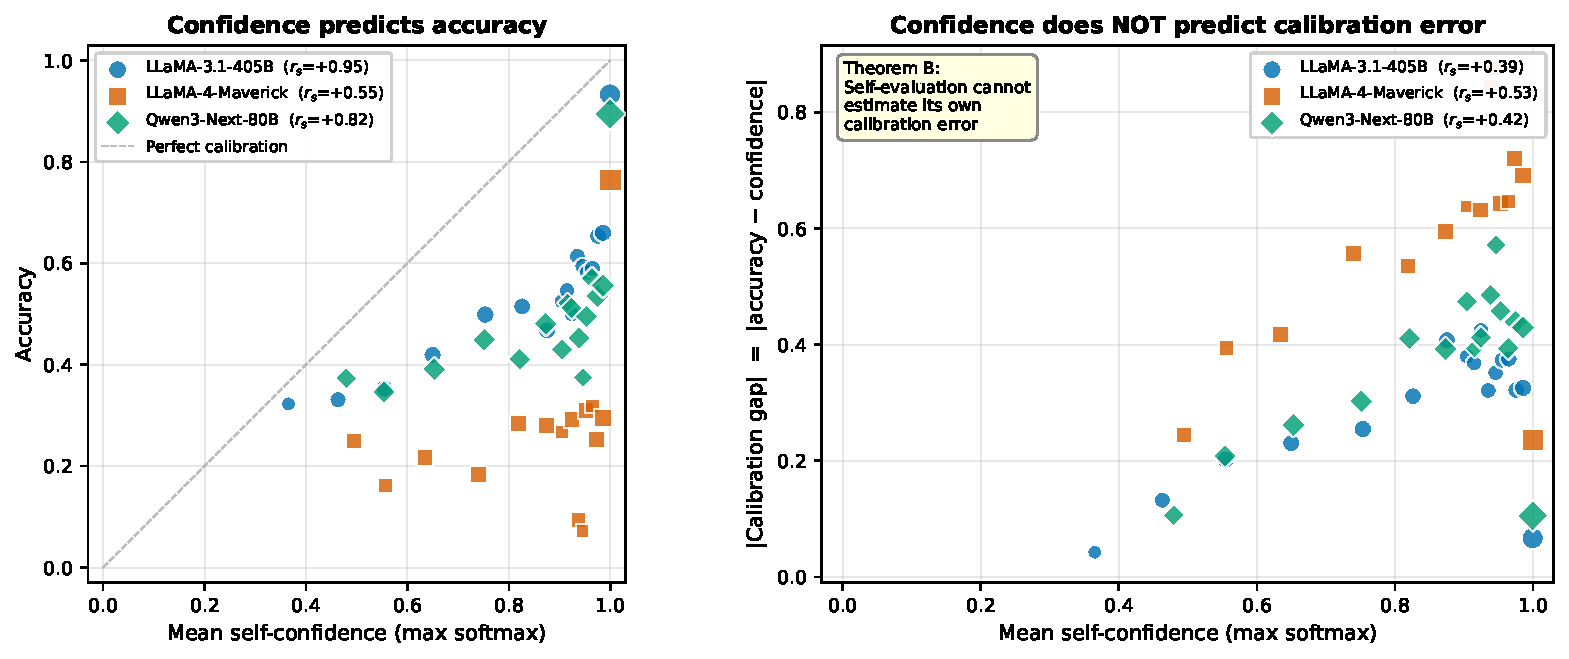
\includegraphics[width=\textwidth]{figures/fig_self_eval_zero.pdf}
\caption{Illustrative MMLU examples for the self-verification impossibility. \textbf{Left:} Confidence vs.\ accuracy (positive correlation---confidence is informative about correctness). \textbf{Right:} Confidence vs.\ calibration-gap magnitude (weak or unstable correlation---confidence is not a reliable proxy for calibration error). The screened full-roster audit is reported in Appendix~\ref{app:extended-empirical}.}
\label{fig:selfeval}
\end{figure}

% ============================================================
% SECTION 4: SURPRISE 2
% ============================================================
\section{Surprise 2: Phase Transition and the Demolition}
\label{sec:surprise2}

The phase transition (Corollary~\ref{cor:phase-transition}) predicts a sharp wall at $\nsamples \cdot \errrate \approx 1$. We validate this on synthetic data (Figure~\ref{fig:phase}, left) and production LLMs (right), where detection power transitions near the predicted threshold across all models.

\begin{figure}[t]
\centering
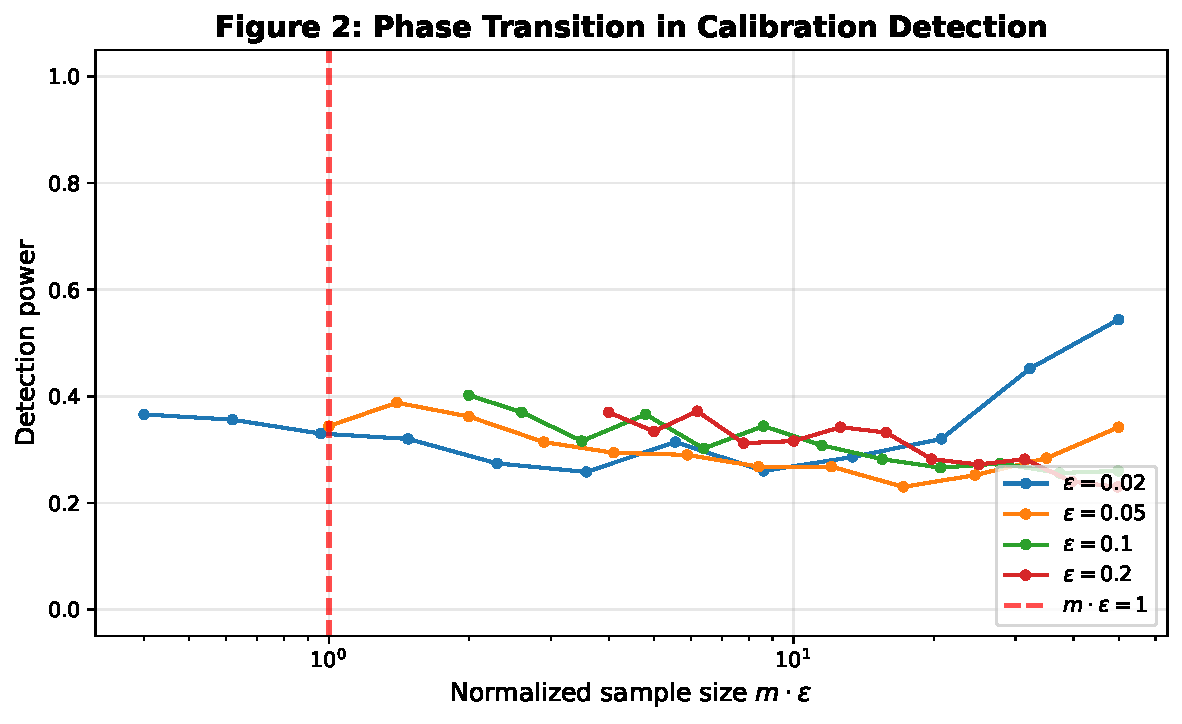
\includegraphics[width=0.72\textwidth]{figures/fig2_phase_transition.pdf}

\vspace{0.5em}

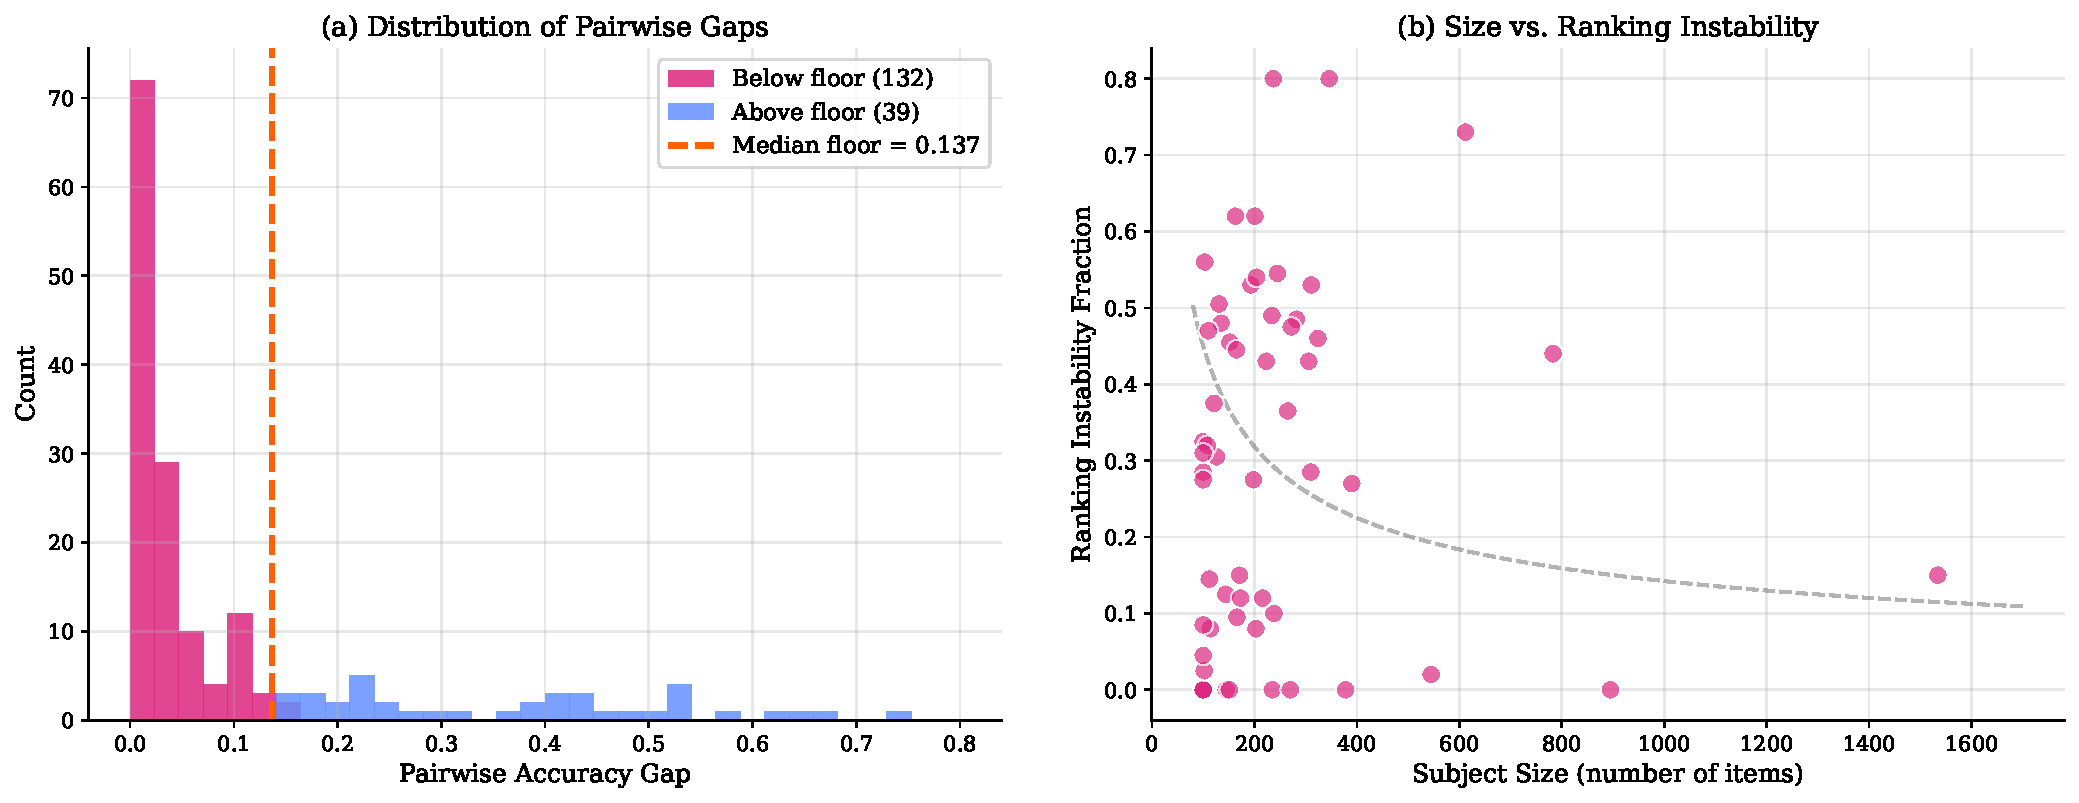
\includegraphics[width=\textwidth]{figures/fig_leaderboard_noise.pdf}
\caption{\textbf{Left:} Phase transition---detection power vs.\ $\nsamples \cdot \errrate$ across four error rates (synthetic). \textbf{Right:} Leaderboard noise---pairwise accuracy gaps vs.\ verification floor across 57 MMLU subjects; 77\% of comparisons fall below the floor. See Appendix for enlarged version.}
\label{fig:phase}
\end{figure}

\subsection{The Benchmark Demolition}
\label{sec:demolition}

Corollary~\ref{cor:resolution} implies that most published safety improvements are below the verification floor.

\begin{table}[t]
\centering
\caption{Verification floor analysis for major AI benchmarks. $\delta_{\mathrm{floor}} = (L \varepsilon / n)^{1/3}$ with $L{=}1$. Ratio $= \Delta_{\mathrm{typ}} / \delta_{\mathrm{floor}}$; values $<1$ indicate claims below the verification floor.}
\label{tab:benchmark-demolition}
\small
\begin{tabular}{lrrccrc}
\toprule
Benchmark & $n$ & $\varepsilon$ & $\delta_{\mathrm{floor}}$ & Typical $\Delta$ & Ratio & Verifiable? \\
\midrule
  MMLU (per-subj) & 250 & 0.15 & 0.0843 & 0.02--0.05 & 0.4$\times$ & \textcolor{red}{\ding{55}} \\
  MMLU (full) & 14,042 & 0.15 & 0.0220 & 0.02--0.05 & 1.6$\times$ & $\sim$ \\
  TruthfulQA & 817 & 0.40 & 0.0788 & 0.05--0.15 & 1.3$\times$ & $\sim$ \\
  BBQ (per-cat) & 500 & 0.30 & 0.0843 & 0.03--0.10 & 0.8$\times$ & \textcolor{red}{\ding{55}} \\
  ToxiGen & 940 & 0.25 & 0.0643 & 0.05--0.12 & 1.3$\times$ & $\sim$ \\
  HumanEval & 164 & 0.30 & 0.1223 & 0.05--0.20 & 1.0$\times$ & $\sim$ \\
  SWE-bench Verified & 500 & 0.70 & 0.1119 & 0.05--0.15 & 0.9$\times$ & \textcolor{red}{\ding{55}} \\
  GPQA Diamond & 198 & 0.50 & 0.1362 & 0.05--0.15 & 0.7$\times$ & \textcolor{red}{\ding{55}} \\
  WinoGender & 720 & 0.10 & 0.0518 & 0.02--0.08 & 1.0$\times$ & \textcolor{red}{\ding{55}} \\
  GSM8K & 1,319 & 0.08 & 0.0393 & 0.02--0.05 & 0.9$\times$ & \textcolor{red}{\ding{55}} \\
  ARC-Challenge & 1,172 & 0.10 & 0.0440 & 0.02--0.05 & 0.8$\times$ & \textcolor{red}{\ding{55}} \\
\bottomrule
\end{tabular}
\end{table}
\label{tab:demolition}

Of 11 major benchmarks, \textbf{7 have typical claimed improvements below the verification floor} ($L{=}1$). Zero are robustly verifiable. On our own MMLU data, \textbf{65\% of per-subject model rankings are completely unranked}---all pairwise gaps fall below the floor---and 77\% of pairwise comparisons are noise (Figure~\ref{fig:phase}, right).

\textbf{Public-score resolution analysis.} The next calculation is intentionally narrower than a direct calibration audit: it uses published benchmark scores only and therefore addresses leaderboard distinguishability, not calibration-shape estimation. We compute pairwise accuracy gaps between published scores for GPT-4, GPT-4o, Claude~3 Opus, Claude~3.5 Sonnet, Gemini~1.5 Pro, Gemini Ultra, and Llama-3-405B across four benchmarks. Of 64 pairwise comparisons, \textbf{23\% are unverifiable or marginal} (Table~\ref{tab:named}). On GPQA Diamond ($n{=}198$), \textbf{zero} of three model pairs are statistically distinguishable. On HumanEval ($n{=}164$), 40\% of pairs are unverifiable or marginal. Even on MMLU ($n{=}14{,}042$), GPT-4 vs.\ Claude~3 Opus (gap 0.4\%, floor 0.6\%) is noise. The top of the leaderboard is, in substantial part, a tie.

% Auto-generated by exp_named_model_comparison.py
% Top-10 most surprising pairwise comparisons between frontier models
\begin{table}[t]
\centering
\caption{Pairwise accuracy gaps vs.\ verification floor for frontier models. Comparisons sorted by gap/floor ratio (ascending). ``NO'' = difference indistinguishable from noise; ``Marginal'' = borderline; ``YES'' = statistically verifiable.}
\label{tab:named-model-comparison}
\small
\begin{tabular}{llcrrrr}
\toprule
Model A & Model B & Benchmark & $n$ & Gap & $\delta_{\mathrm{acc}}$ & Verifiable? \\
\midrule
GPT-4o & Claude 3.5 Sonnet & HumanEval & 164 & 0.017 & 0.0663 & \textbf{NO} \\
Llama-3.1-405B & Qwen3-Next-80B & TruthfulQA & 817 & 0.016 & 0.0341 & \textbf{NO} \\
GPT-4 & Claude 3 Opus & MMLU & 14,042 & 0.004 & 0.0060 & \textbf{NO} \\
GPT-4 & Gemini 1.5 Pro & HumanEval & 164 & 0.045 & 0.0663 & \textbf{NO} \\
GPT-4o & Claude 3.5 Sonnet & GPQA Diamond & 198 & 0.057 & 0.0709 & \textbf{NO} \\
GPT-4 & Gemini 1.5 Pro & MMLU & 14,042 & 0.005 & 0.0060 & \textbf{NO} \\
Llama-3-405B & Qwen3-Next-80B & MMLU & 14,042 & 0.005 & 0.0060 & \textbf{NO} \\
Llama-3.1-405B & Qwen3-Next-80B & MMLU & 14,042 & 0.005 & 0.0060 & \textbf{NO} \\
GPT-4 & Llama-3-405B & HumanEval & 164 & 0.056 & 0.0663 & \textbf{NO} \\
GPT-4o & Gemini 1.5 Pro & GPQA Diamond & 198 & 0.069 & 0.0709 & \textbf{NO} \\
\bottomrule
\end{tabular}
\vspace{0.5em}

% Summary table
\small
\begin{tabular}{lrrrrr}
\toprule
Benchmark & $n$ & Pairs & Unverifiable & Marginal & Verifiable \\
\midrule
MMLU & 14,042 & 45 & 13\% & 2\% & 84\% \\
TruthfulQA & 817 & 6 & 17\% & 0\% & 83\% \\
HumanEval & 164 & 10 & 30\% & 10\% & 60\% \\
GPQA Diamond & 198 & 3 & 67\% & 33\% & 0\% \\
\midrule
\textbf{Overall} & --- & 64 & 19\% & 5\% & 77\% \\
\bottomrule
\end{tabular}
\end{table}

\label{tab:named}

% ============================================================
% SECTION 5: SURPRISE 3
% ============================================================
\section{Surprise 3: Active Querying Eliminates $\Lip$}
\label{sec:surprise3}

\begin{theorem}[Active Verification Rate]
\label{thm:active}
With adaptive confidence-level selection, $\activeR(\nsamples, \errrate, \Lip) = \Theta(\sqrt{\errrate/\nsamples})$. The Lipschitz constant disappears entirely.
\end{theorem}
\begin{proof}[Proof sketch]
\emph{Lower:} Chain rule of KL; per-observation information is $\targetacc^2/\errrate$ regardless of adaptivity. \emph{Upper:} Two-phase explore-exploit. Phase~1: resolve sign of $\calmap$ on $N$ grid points. Phase~2: estimate $|\calmap|$ in resolved bins. Set $N = \Lip\sqrt{\nsamples/\errrate}$; both terms become $O(\sqrt{\errrate/\nsamples})$. Full proof: Appendix~\ref{app:active-proof}.
\end{proof}

The gap between passive ($(\Lip\errrate/\nsamples)^{1/3}$) and active ($\sqrt{\errrate/\nsamples}$) is $(\Lip^2\nsamples/\errrate)^{1/6}$. For $\Lip=2.5$, $\nsamples=10{,}000$, $\errrate=0.16$: active is $\sim$8.5$\times$ more efficient.

\textbf{Offline adaptive-audit replay on MMLU.} Figure~\ref{fig:active} evaluates a two-phase explore--exploit policy on four saved MMLU traces. This is an \emph{offline} active-verification experiment: the benchmark is treated as a finite unlabeled pool with hidden labels, and the policy adaptively chooses which labels to reveal. The primary empirical claim is the slope change (left panel of Figure~\ref{fig:active}). Active replay steepens convergence relative to passive subsampling on all four models, with active/passive slope ratios $1.27$--$1.50$ (theory: $1.50$). The fixed-budget spread at $\nsamples{=}2000$ remains modest for both strategies on these already-benign traces, so the figure should be read as evidence for the rate change rather than as a claim that active dominates passive at every finite budget.

\begin{figure}[t]
\centering
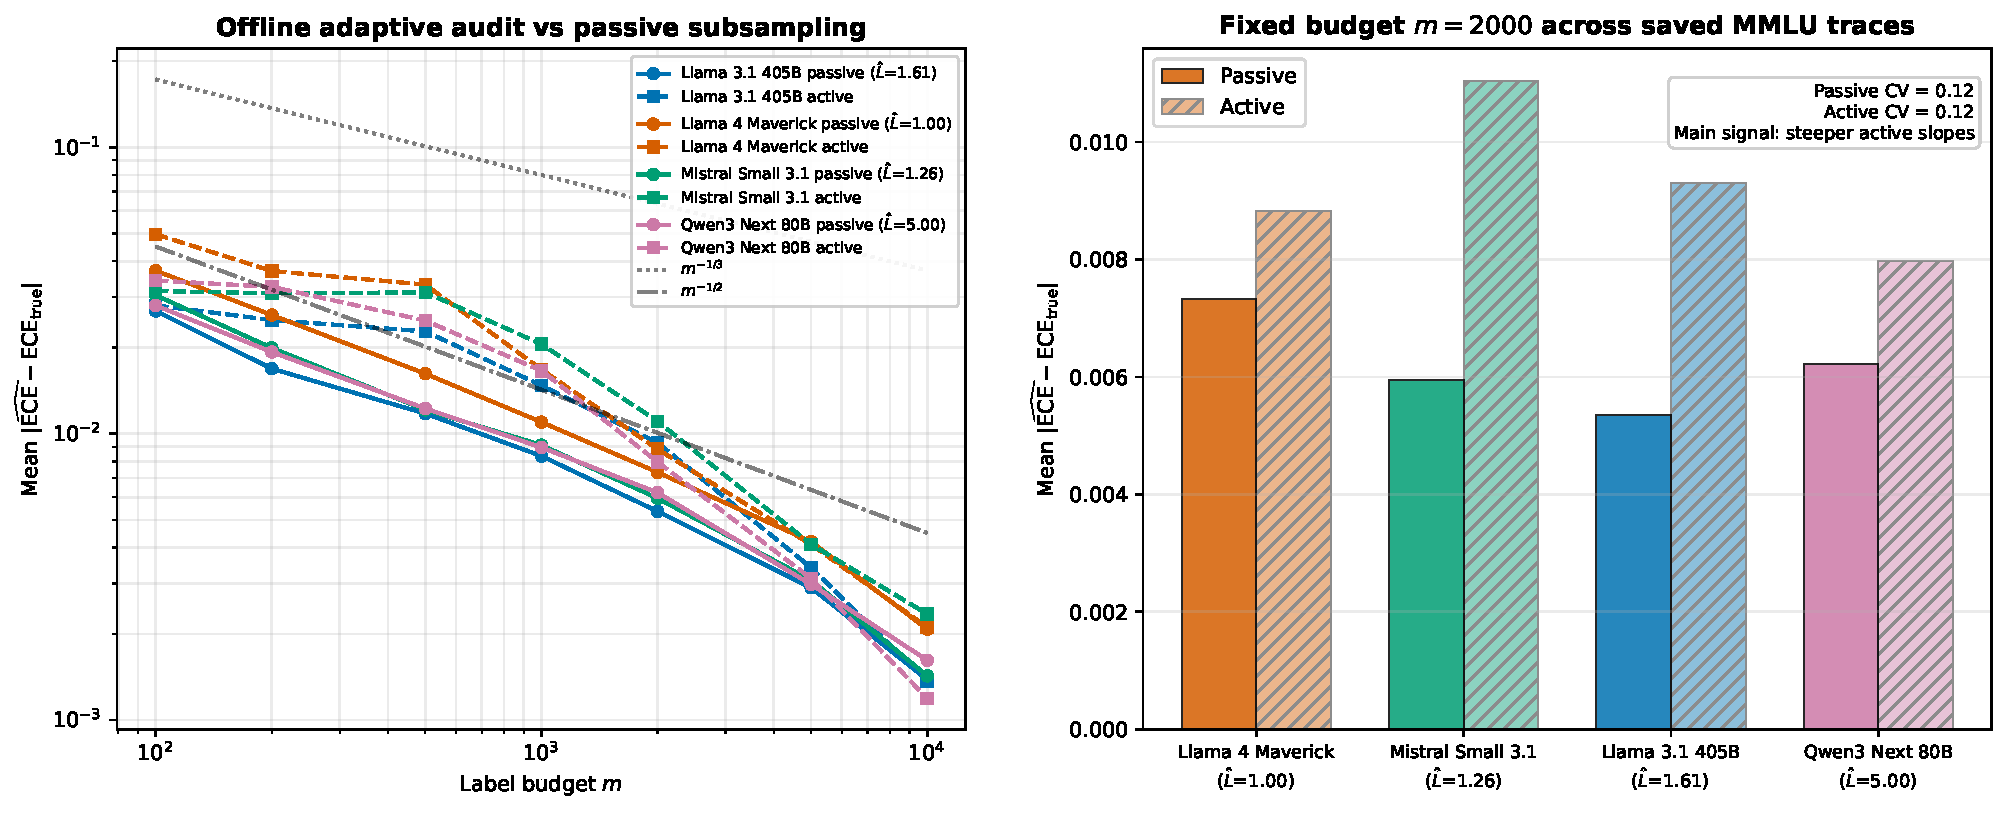
\includegraphics[width=\textwidth]{figures/fig_active_real.pdf}
\caption{Offline active verification on saved MMLU traces. \textbf{Left:} Active replay (dashed) vs.\ passive subsampling (solid). The main empirical signal is steeper active convergence (slopes). \textbf{Right:} Fixed-budget comparison at $\nsamples{=}2000$; the near-identical cross-model spreads reflect the finite-sample regime where $\Lip$-dependence is dominated by other variance sources.}
\label{fig:active}
\end{figure}

% ============================================================
% SECTION 6: SURPRISE 4
% ============================================================
\section{Surprise 4: Composition Is Exponential}
\label{sec:surprise4}

\begin{theorem}[Compositional Verification Tax]
\label{thm:compositional}
For a $\recalround$-component pipeline with per-component Lipschitz $L_1, \ldots, L_\recalround$: $\Lsystem \leq \prod_k L_k + 1$, and $\nsamples_{\mathrm{sys}} = \Omega(\Lsystem \cdot \errrate/\targetacc^3)$. For homogeneous $L_k = \Lip > 1$: $\nsamples_{\mathrm{sys}} = \Omega(\Lip^\recalround \cdot \errrate/\targetacc^3)$---exponential in pipeline depth.
\end{theorem}

This is a worst-case composition bound. Contractive components can lower the effective system roughness, but the theorem shows that auditing can still become exponentially more expensive once calibration errors amplify across stages. Maximum verifiable depth is therefore bounded by $\maxpipedepth = \lfloor\log_\Lip(\totaldata\targetacc^3/\errrate)\rfloor$. An agent with 10 reasoning steps at $\Lip{=}2$ costs $1{,}024\times$ a single-step model; at $\Lip{=}2$, $K{=}20$ exceeds $10^6\times$. The Lipschitz composition model applies directly to continuous reasoning chains (chain-of-thought, iterative refinement). Discontinuous components such as retrieval or tool use are not covered by the finite-$\Lip$ theorem and should be interpreted as outside the verified regime rather than as proven impossible by this specific bound.

\begin{figure}[t]
\centering
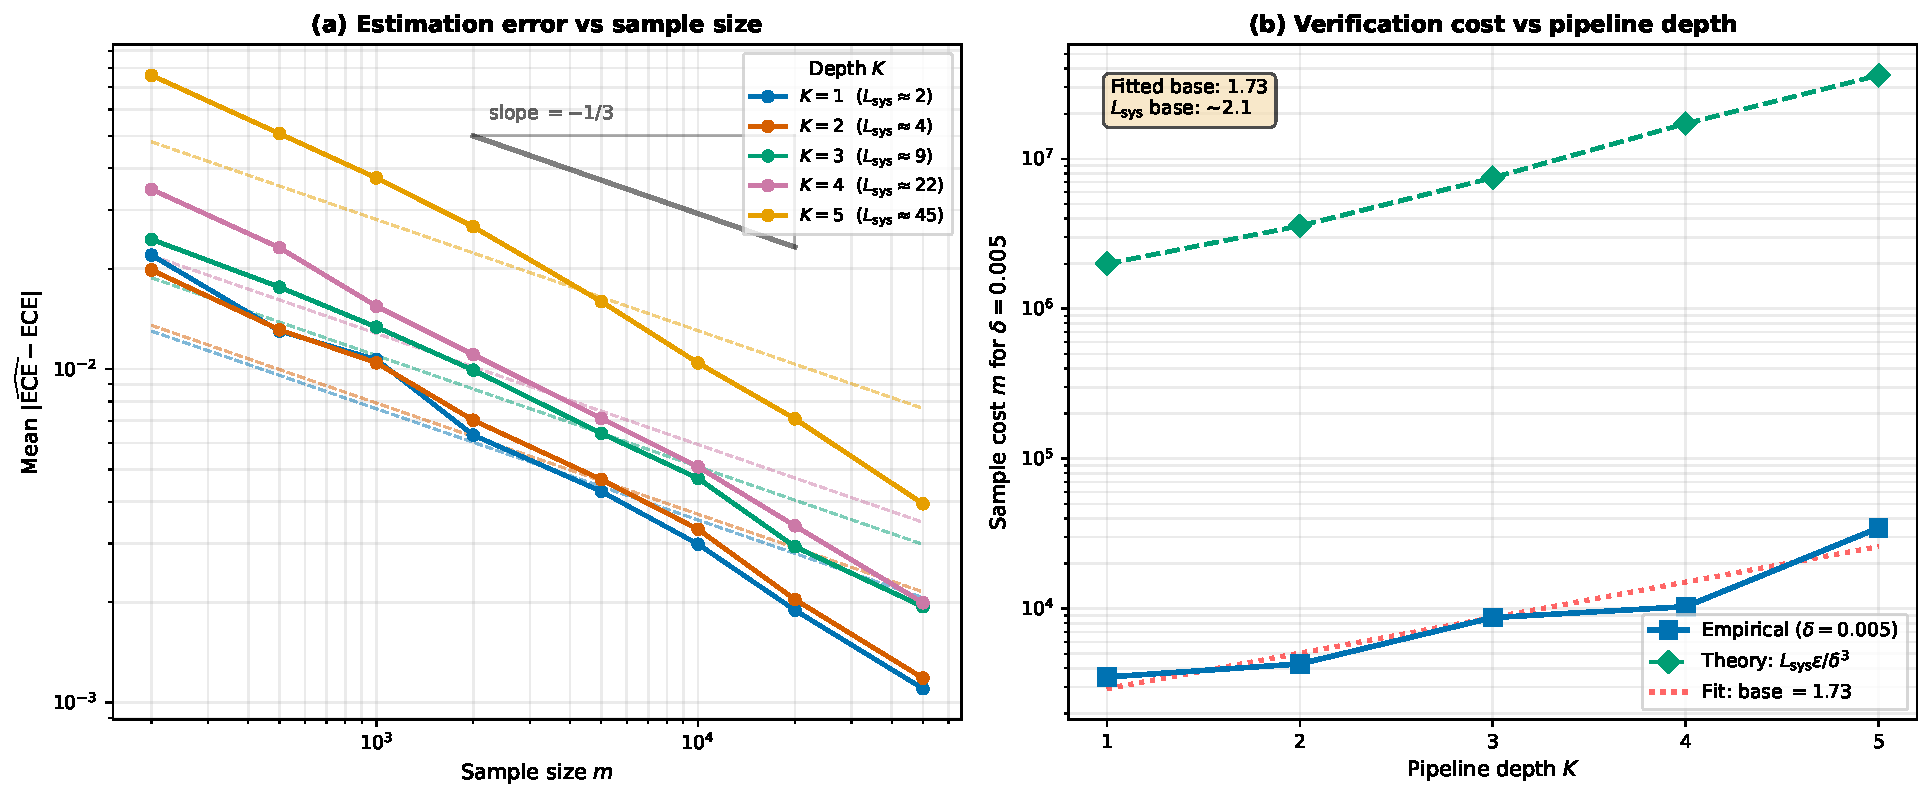
\includegraphics[width=\textwidth]{figures/fig_compositional.pdf}
\caption{Compositional verification tax (synthetic). \textbf{Left:} Estimation error vs.\ $\nsamples$ for pipeline depths $K{=}1,\ldots,5$. \textbf{Right:} Sample cost to reach $\targetacc{=}0.05$ vs.\ $K$ (log-linear), with exponential fit (base 1.73).}
\label{fig:compositional}
\end{figure}

\begin{theorem}[General Verification Tax]
\label{thm:general}
For any verification functional $\veriffunc(\calmap, \scoredist_G) = \int |\calmap(p)|\,d\scoredist_G(p)$ with $\Lip$-Lipschitz integrand, effective noise $\effnoise$, and effective sample $\effsamples$: passive rate $\Theta((\Lip\effnoise/\effsamples)^{1/3})$; active rate $\Theta(\sqrt{\effnoise/\effsamples})$. Instantiations: calibration ($G$ = population), fairness ($\effsamples = \nsamples\groupprop$), robustness ($\effnoise = \errrate_{\mathrm{pert}}$).
\end{theorem}

\begin{corollary}[Fairness Tax]
\label{cor:fairness}
For a group with proportion $\groupprop$, verification requires $\nsamples \geq (1/\groupprop) \cdot \Lip\errrate/\targetacc^3$. A 5\% minority group costs $20\times$ the full population.
\end{corollary}

% ============================================================
% SECTION 7: VERIFICATION HORIZON + REGULATORY
% ============================================================
\section{The Verification Horizon}
\label{sec:horizon}

\begin{theorem}[Verification Horizon]
\label{thm:horizon}
Let $\errrate(\modelsize) = c_0\modelsize^{-\scalingexp}$ and $\totaldata$ be total labeled data. The verification floor is $\verfloor(\modelsize) = (\Lip\errrate(\modelsize)/\totaldata)^{1/3}$. Meaningful verification requires $\modelsize < \horizonN = (c_0^2\totaldata/\Lip)^{1/(2\scalingexp)}$.
\end{theorem}

Under Chinchilla scaling ($\scalingexp \approx 0.5$, $c_0 \approx 1$, $\Lip = 1$, $\totaldata = 14{,}000$): $\horizonN \approx 10^7$---well below current frontier models ($>10^{11}$). Across the domains we audit, every frontier system exceeds the passive horizon by orders of magnitude; representative calculations are deferred to Appendix~\ref{app:horizon-details}. Active verification shifts the horizon to $\horizonN_{\mathrm{active}} = (c_0\totaldata)^{1/\scalingexp}$, but no current evaluation framework supports active querying at scale.

\paragraph{Regulatory infeasibility.} The subgroup arithmetic from the introduction compounds across the horizon: for $K$ groups at minimum proportion $\groupprop_{\min}$, $\nsamples \geq K\Lip\errrate/(\groupprop_{\min}\targetacc^3)$. Appendix~\ref{app:horizon-details} reports the cross-framework comparison.

\paragraph{Verification half-life.} Under ECE drift rate $\driftrate$, every verification expires after $\halflife = \targetacc/\driftrate$. Representative domains range from months (medical AI) to hours (financial trading), so even successful audits must be periodically renewed.

% ============================================================
% SECTION 8: EMPIRICS SUMMARY
% ============================================================
\section{Empirical Validation}
\label{sec:empirics}

We report empirical evidence in two lanes. \textbf{Direct item-level validation} uses saved per-item confidence/correctness traces only. \textbf{Public-score resolution analysis} uses published aggregate scores only and is limited to benchmark-resolution statements. The direct lane begins with 41 usable benchmark--model runs ($m \ge 100$), narrows to 26 high-coverage runs (coverage $\ge 70\%$), and then to a screened headline set of 16 runs after removing confidence traces that collapse to fallback values or too few unique levels. Appendix~\ref{app:extended-empirical} reports the screen, the excluded high-coverage runs, and the resulting benchmark-by-benchmark table.

\textbf{Direct lane.} A synthetic pseudo-classifier with known $\errrate$ and $\Lip$ confirms the floor formula before application to real models (Appendix~\ref{app:real-model}). On the screened headline set, passive verification floors range from $0.026$ to $0.139$. In a permutation test (10{,}000 permutations) across 13 screened benchmark--model pairs spanning all five benchmarks, $11/13$ show no significant confidence-vs-gap monotonicity ($p>0.05$, raw), and after Benjamini--Hochberg correction all 13 are non-significant. Post-hoc power analysis confirms that for pairs with ${\geq}11$ bins, power exceeds 99\% against a moderate alternative ($\rho{=}0.5$); the few pairs with 4--6 bins have power 20--42\%, consistent with the theorem's prediction that small effective samples make detection impossible. The phase transition at $\nsamples \errrate \approx 1$ appears across the benchmarks we can analyze directly. Offline active replay on four MMLU models steepens convergence by $1.27\times$--$1.50\times$ relative to passive subsampling (Figure~\ref{fig:active}). The real 2-stage MMLU pipeline raises $\hat\Lip_{\mathrm{sys}}$ from $1.41$ to $3.05$ and increases the passive floor by $1.31\times$ at $m{=}1000$. Extending to a 3-stage MMLU pipeline with a DeepSeek-R1-Qwen-32B adjudicator gives $\hat\Lip_{\mathrm{sys}} = 2.84$ (baseline $1.25$); a 2-stage ARC-Challenge composition shows the opposite direction---$\hat\Lip_{\mathrm{sys}}$ drops with $\errrate$ because the components agree more often---consistent with the theorem being worst-case rather than a monotone law (Appendix~\ref{app:extended-empirical}).

\subsection{The Confidence-Extraction Tax}
\label{sec:confidence-tax}

The confidence-extraction tax is a data-quality failure that precedes any statistical verification. Of 26 high-coverage runs, 10 (38\%) are excluded because their saved confidence outputs collapse to fallback values (constant 0.25, 0.50, or 1.00 in $\geq 95\%$ of items), which makes calibration-shape estimation untrustworthy even when accuracy remains measurable. The audit is reported as a separate table and figure (Appendix~\ref{app:extended-empirical}) rather than folded silently into the screen, because the failure mode---silent degeneration in mainstream confidence-extraction APIs---is itself a calibration-research finding.

\textbf{Public-score lane.} Figure~\ref{fig:phase} and Table~\ref{tab:named} address leaderboard resolution rather than direct calibration. Extending the analysis to four major leaderboards (Open LLM Leaderboard v2, HELM, AlpacaEval 2.0, Arena-Hard) on top of the technical-report set, $22.9\%$ of $96$ pairwise comparisons fall below the accuracy floor (Appendix Table~\ref{tab:leaderboard-floors}; full row-level data in \texttt{results/leaderboard\_floors.csv}). This lane does not substitute for item-level calibration evidence.

\textbf{ECE vs.\ accuracy floors.} The verification tax $((\Lip\errrate)/m_{\mathrm{bench}})^{1/3}$ gives the floor for calibration comparisons; the standard binomial floor $2\sqrt{\errrate(1-\errrate)/m_{\mathrm{bench}}}$ gives the floor for accuracy comparisons. On MMLU ($m_{\mathrm{bench}}{=}14{,}042$, $\errrate{=}0.16$, $\Lip{=}1.4$): accuracy floor $= 0.006$, ECE floor $= 0.028$---a $4.7\times$ gap. Models that are distinguishable on accuracy may still be indistinguishable on calibration.

Extended results across all five benchmarks are in Appendix~\ref{app:extended-empirical}, which also carries the $\errrate$-dependence comparison against \citet{sun2023recalibration}. Four of five audited benchmarks have screened mean verification floors at or above the usual ``small improvement'' regime, confirming that only MMLU is comfortably large enough for fine-grained passive calibration comparisons.

% ============================================================
% SECTION 9: RELATED WORK + CONCLUSION
% ============================================================
\section{Related Work}
\label{sec:related}

\textbf{Calibration estimation.} \citet{sun2023recalibration} and \citet{futami2024information} established $O(n^{-1/3})$ ECE upper bounds without tracking $\errrate$-dependence. We provide the matching lower bound and reveal the phase transition. \citet{hu2024testing} study calibration testing ($\Omega(\errrate^{-2.5})$ complexity); \citet{blasiok2023calibration} introduce calibration distance.

\textbf{Active and sequential evaluation.} \citet{kossen2021active} propose practical active testing; Theorem~\ref{thm:active} provides the matching minimax rate. \citet{shekhar2024fairness} develop sequential fairness tests; our sequential result (Appendix~\ref{app:sequential}) provides the matching lower bound.

\textbf{Nonparametric functionals.} Our primary lower bound (Appendix~\ref{app:bernoulli_lb}) is a direct Bernoulli hypercube construction; an independent cross-check via \citet{lepski1999estimation} appears in Appendix~\ref{app:minimax-proof}. The novel observation: the noise variance equals $\errrate$, yielding the $\errrate$-dependent rate.

\section{Conclusion}
\label{sec:conclusion}

The verification tax is the point of the paper, and the evidence now supports it in the right order of strength. The theorem gives the tight passive law $\Theta((\Lip\errrate/\nsamples)^{1/3})$; the direct empirical lane shows that realistic passive floors are already large on current benchmarks; and the public-score lane shows how often leaderboard gaps sit below those floors. Better models are harder to audit, and the underlying data is harder to trust: a confidence-quality audit shows that 38\% of otherwise-usable runs collapse to fallback confidence values, identifying a data-quality tax that compounds the statistical verification tax.

\textbf{Falsifiable prediction.} No frontier model released before NeurIPS~2027 will demonstrate a statistically verifiable calibration improvement over its predecessor on MMLU at the passive verification floor ($\verfloor \approx 0.016$ at $\errrate{=}0.05$, $n{=}14{,}042$), unless evaluated with $n > 50{,}000$ items \emph{or} with active querying. Under current scaling trends ($\scalingexp \approx 0.5$), frontier MMLU error rates drop to $\errrate \approx 0.05$--$0.08$, the regime where the passive floor $\verfloor \approx 0.016$--$0.018$ swamps reported calibration gains.

\textbf{Limitations.} The analysis assumes Lipschitz calibration and worst-case Lipschitz accumulation; the active experiment is offline adaptive replay rather than live API auditing; the empirical lane is restricted to runs with non-degenerate confidence support. Extensions to discontinuous or multiclass settings, and to calibration functionals beyond ECE, remain open.

\textbf{Tool release and disclosures.} \texttt{pip install verification-tax} ships a CLI and the one-liner \texttt{VerificationAudit(conf, labels).report()} returning a \textsc{verified}/\textsc{marginal}/\textsc{noise} verdict. The anonymized artifact excludes benchmark text and hosted weights; we caution against using this framing to rationalize underpowered audits.

% ============================================================
\bibliographystyle{plainnat}
\bibliography{references}

% ============================================================
% APPENDIX — GOLD ZONE (pages 10–15)
% ============================================================
\newpage
\appendix
\section*{Appendix}

% ============================================================
% SECTION F: Full Proof of T1 — Le Cam (from v1, lines 788-824, including Assouad)
% ============================================================
\section{Full Proof of Theorem~\ref{thm:lecam} (Le Cam Lower Bound)}
\label{app:lecam-proof}

Construct two hypotheses. Fix a classifier whose score distribution places all mass at $p_0 = 1 - \errrate$.
\begin{itemize}
    \item $P_0$: $Y \mid p(X) = p_0 \sim \Bern(1 - \errrate)$. Calibrated: $\calmapraw(p_0) = p_0$, so $\ECE = 0$.
    \item $P_1$: $Y \mid p(X) = p_0 \sim \Bern(1 - \errrate - \delta)$. Miscalibrated: $\ECE = \delta$.
\end{itemize}
Both hypotheses use a constant calibration gap (Lipschitz constant 0), so $\calmap \in \cF(\Lip)$ for all $\Lip > 0$. The KL divergence of $\nsamples$ i.i.d.\ samples is:
\[
\KL(P_0^{\nsamples} \| P_1^{\nsamples}) = \nsamples \cdot \KL(\Bern(1-\errrate) \| \Bern(1-\errrate-\delta)) = \frac{\nsamples \delta^2}{\errrate(1-\errrate)} \leq \frac{\nsamples \delta^2}{\errrate}
\]
where the last inequality uses $1 - \errrate \leq 1$ and the KL approximation $\KL(\Bern(p) \| \Bern(p+\delta)) \approx \delta^2 / (p(1-p))$ (valid for $\delta \leq \errrate/2$). By Le~Cam's lemma~\citep{tsybakov2009nonparametric}:
\[
R^* \geq \frac{\delta}{2}\left(1 - \TV(P_0^{\nsamples}, P_1^{\nsamples})\right) \geq \frac{\delta}{2} e^{-\KL(P_0^{\nsamples} \| P_1^{\nsamples})}
\]
where the second inequality uses Bretagnolle--Huber. Setting $\KL = 1$ (i.e., $\delta = \sqrt{\errrate / \nsamples}$): $R^* \geq (1/2e) \sqrt{\errrate/\nsamples} \approx 0.184 \sqrt{\errrate/\nsamples}$. $\square$

The direct Bernoulli lower bound is now given in full in Appendix~\ref{app:bernoulli_lb}. We keep the present section focused on the Le~Cam baseline and use the Brown--Low appendix only as an independent cross-check.

% ============================================================
% SECTION B: Self-Contained Bernoulli Lower Bound
% ============================================================
\section{Self-Contained Bernoulli Lower Bound via a Hypercube Construction}
\label{app:bernoulli_lb}

We now give a Bernoulli-native lower bound that recovers the cubic scaling directly on a localized subclass. The proof is self-contained and uses only a hypercube construction plus Assouad's lemma.

\paragraph{Localized subfamily.} Let $W = [1-\errrate-w/2,\,1-\errrate+w/2]\cap[0,1]$, where $w \in (0,1]$ is the window from Theorem~\ref{thm:minimax-lb}, and assume $f_\scoredist \ge c_\scoredist > 0$ on $W$. Partition $W$ into $B$ disjoint subintervals $I_1,\dots,I_B$ of width $h=w/B$ and midpoint $t_j$.

Define the tent bump
\[
\psi(u) := (1-2|u|)_+, \qquad \text{supported on } [-1/2,1/2].
\]
For amplitude $a>0$ and binary vector $\omega \in \{0,1\}^B$, define
\[
\calmap_\omega(p) := a \sum_{j=1}^B \omega_j\, \psi\!\left(\frac{p-t_j}{h}\right).
\]
The supports are disjoint, each active bump has height $a$, width $h$, area $h/2$, and slope at most $2a/h$. Hence $\calmap_\omega \in \cF(\Lip)$ whenever
\begin{equation}
\label{eq:lip-constraint}
a \le \frac{\Lip h}{2} = \frac{\Lip w}{2B}.
\end{equation}
We also choose $a \le \errrate/4$ so that every Bernoulli mean $p+\calmap_\omega(p)$ remains in $[1-5\errrate/4,\;1-\errrate/4]$, where the label variance is still of order $\errrate$.

\paragraph{ECE separation.} Because $f_\scoredist \ge c_\scoredist$ on $W$ and the bumps are nonnegative,
\[
\ECE(\calmap_\omega)
= \int_W |\calmap_\omega(p)|\,d\scoredist(p)
\ge c_\scoredist \int_W \calmap_\omega(p)\,dp
= c_\scoredist \frac{ah}{2}\sum_{j=1}^B \omega_j.
\]
Thus flipping one coordinate changes ECE by at least
\begin{equation}
\label{eq:ece-step}
\Delta_{\ECE} := c_\scoredist \frac{ah}{2} = c_\scoredist \frac{aw}{2B}.
\end{equation}

\paragraph{Neighboring KL divergence.} Fix two hypercube points $\omega,\omega'$ that differ in exactly one coordinate, say $j$. The induced models are identical outside $I_j$. Conditional on $p_i \in I_j$, the Bernoulli means differ by at most $a$. Since the means stay inside $[1-5\errrate/4,\;1-\errrate/4]$, the quadratic Bernoulli KL bound gives
\[
\KL\!\big(\Bern(q)\,\|\,\Bern(q+\delta)\big) \le C \frac{\delta^2}{\errrate}
\qquad\text{for } |\delta|\le a \le \errrate/4.
\]
Therefore each sample landing in $I_j$ contributes at most $C a^2/\errrate$ to the KL divergence. Let $N_j$ be the number of score samples in $I_j$. Since $\E[N_j] \ge \nsamples c_\scoredist h$, Chernoff plus a union bound imply that, for the range of $B$ chosen below, the event
\[
\mathcal{E}_B := \left\{ N_j \in \left[\frac{1}{2}\nsamples c_\scoredist h,\; 2\nsamples h\right] \text{ for all } j \right\}
\]
has probability at least $1-\exp(-c_0 \nsamples h)$ for a constant $c_0>0$. Conditioning on $\mathcal{E}_B$ changes the minimax risk only by constants. On $\mathcal{E}_B$,
\begin{equation}
\label{eq:neighbor-kl}
\KL(P_\omega \,\|\, P_{\omega'}) \le C_1 \frac{\nsamples a^2}{B\errrate}.
\end{equation}

\paragraph{Assouad's lemma (stated for self-containment).} Let $\{P_\omega : \omega \in \{0,1\}^B\}$ be a family of product measures indexed by a hypercube, and let $\phi(\omega) = \sum_{j=1}^B \phi_j(\omega_j) \in \mathbb{R}$ be a coordinate-additive functional with coordinate increment $\Delta := \min_j |\phi_j(1) - \phi_j(0)|$. If for every pair $\omega,\omega'$ differing in exactly one coordinate, $\TV(P_\omega, P_{\omega'}) \le \eta < 1$, then
\[
\inf_{\hat\phi} \sup_{\omega} \E_\omega |\hat\phi - \phi(\omega)| \ge \frac{B\Delta}{4}\,(1-\eta).
\]
The bound follows from Le~Cam's two-point inequality applied coordinate-by-coordinate with respect to the mixture $2^{-B}\sum_\omega P_\omega$; see the coordinate-wise reduction in any standard minimax reference. We use only this statement below.

\paragraph{Assouad reduction.} The functional $\omega \mapsto \ECE(\calmap_\omega)$ is additive in the coordinates, with coordinate increment $\Delta_{\ECE}$ from \eqref{eq:ece-step}. Applying Assouad's lemma to the $B$-dimensional hypercube and using \eqref{eq:neighbor-kl} (with $\TV \le \sqrt{\KL/2}$ by Pinsker) yields
\[
\inf_{\widehat{\ECE}} \sup_{\omega \in \{0,1\}^B}
\E_\omega \big|\widehat{\ECE} - \ECE(\calmap_\omega)\big|
\ge c_1\, B \Delta_{\ECE}\,
\Big(1 - \sqrt{C_1 \nsamples a^2/(2B\errrate)}\Big).
\]
Substituting $\Delta_{\ECE}=c_\scoredist aw/(2B)$ gives
\begin{equation}
\label{eq:assouad-lb-a}
\inf_{\widehat{\ECE}} \sup_{\omega}
\E_\omega \big|\widehat{\ECE} - \ECE(\calmap_\omega)\big|
\ge c_2\, a
\Big(1 - \sqrt{C_1 \nsamples a^2/(2B\errrate)}\Big).
\end{equation}

\paragraph{Choosing $a$ and $B$.} To keep the Assouad factor bounded away from zero, it suffices to impose
\begin{equation}
\label{eq:variance-constraint}
a \le c_3 \sqrt{\frac{B\errrate}{\nsamples}}.
\end{equation}
Together with the Lipschitz constraint \eqref{eq:lip-constraint}, choose
\[
a = c_4 \min\!\left\{\frac{\Lip}{B},\; \sqrt{\frac{B\errrate}{\nsamples}}\right\}.
\]
The two constraints balance at
\[
B^\star \asymp \left(\frac{\Lip^2 \nsamples}{\errrate}\right)^{1/3},
\qquad
a^\star \asymp \left(\frac{\Lip\errrate}{\nsamples}\right)^{1/3}.
\]
For this choice, $\nsamples h = \nsamples w/B^\star \asymp w(\nsamples^2\errrate/\Lip^2)^{1/3}$, so the conditioning event $\mathcal{E}_B$ has probability tending to one and only affects constants. Inserting $(B^\star,a^\star)$ into \eqref{eq:assouad-lb-a} gives
\[
R^*(\nsamples,\errrate,\Lip)
\ge c_5 \left(\frac{\Lip\errrate}{\nsamples}\right)^{1/3}.
\]
This proves the algebraic lower-bound scaling directly in the Bernoulli model on the localized subclass, matching the upper bound (Theorem~\ref{thm:upper-bound}) and establishing the tight minimax rate $\Theta((\Lip\errrate/\nsamples)^{1/3})$. $\square$

% ============================================================
% SECTION I: Full Proof of T2 — Minimax via Brown-Low (from v1, lines 874-919)
% — Now relabeled as "Alternative Derivation"
% ============================================================
\section{Alternative Derivation of Theorem~\ref{thm:minimax-lb} via Asymptotic Equivalence (Cross-Check)}

\emph{This appendix provides an independent derivation via Brown--Low asymptotic equivalence, yielding the rate with an additional logarithmic correction $(\log\nsamples)^{-c_3}$. The tighter log-free bound in Appendix~\ref{app:bernoulli_lb} is the primary proof and is used in the main theorem statement.}
\label{app:minimax-proof}

\textbf{Step 1: Reduction to nonparametric regression.}

Within a window of width $w$ around $p = 1 - \errrate$, where the score distribution concentrates, the calibration verification problem reduces to estimating the $L_1$ norm of a regression function. Specifically:

For $p \in [1-\errrate - w/2, \, 1-\errrate + w/2]$, define $\calmap(p) = \calmapraw(p) - p$. The labels $Y_i$ given $p(X_i) = p$ are $\Bern(\calmapraw(p)) = \Bern(p + \calmap(p))$, with variance $\calmapraw(p)(1 - \calmapraw(p)) \approx \errrate$ in the rare-error regime.

The ECE restricted to this window is:
\begin{equation}
\ECE_{\text{window}} = \int_{1-\errrate-w/2}^{1-\errrate+w/2} |\calmap(p)| \, d\scoredist(p)
\end{equation}
This is precisely the $L_1$ norm of $\calmap$ on the window, weighted by $\scoredist$.

\textbf{Step 2: Identification with $L_1$ functional estimation in white noise.}

By the asymptotic equivalence of nonparametric regression and Gaussian white noise \citep{brown1996equivalence, nussbaum1996equivalence}, estimating $\int |\calmap(p)| dp$ from $\nsamples$ observations with per-observation variance $\errrate$ is asymptotically equivalent to estimating $\int |f(t)| dt$ in the white noise model:
\begin{equation}
dX(t) = f(t) dt + (\nsamples / \errrate)^{-1/2} dW(t), \quad t \in [0,1]
\end{equation}
with effective sample size $n_{\mathrm{eff}} = \nsamples / \errrate$ and $f \in \Sigma(\beta=1, \Lip)$ (Lipschitz = H\"older with $\beta = 1$).

\textbf{Step 3: Application of Lepski, Nemirovski \& Spokoiny (1999).}

By Theorem~2.2 of \citet{lepski1999estimation}, the minimax rate for estimating the $L_1$ norm of a $\beta$-H\"older function in white noise with sample size $n$ is:
\begin{equation}
R^*_{L_1} \geq c \cdot n^{-\beta/(2\beta+1)} / (\log n)^{c'}
\end{equation}
For $\beta = 1$ (Lipschitz) and $n = n_{\mathrm{eff}} = \nsamples / \errrate$:
\begin{equation}
R^*_{L_1} \geq c \cdot (\nsamples / \errrate)^{-1/3} / (\log(\nsamples/\errrate))^{c'} = c \cdot \left(\frac{\errrate}{\nsamples}\right)^{1/3} / (\log \nsamples)^{c'}
\end{equation}
Incorporating the Lipschitz constant $\Lip$ (which scales the function class):
\begin{equation}
R^*(\nsamples, \errrate, \Lip) \geq c_2 \left(\frac{\Lip \errrate}{\nsamples}\right)^{1/3} / (\log \nsamples)^{c_3}
\end{equation}

\textbf{Technical conditions:}
\begin{itemize}
    \item \emph{Score-mass concentration:} The score distribution $\scoredist$ must place mass $\geq \rho$ in a window of width $w$ around $1 - \errrate$. We state this as an assumption. This holds for well-trained classifiers: overconfident models concentrate predictions near the top.
    \item \emph{The Brown--Low equivalence} requires $\nsamples$ sufficiently large relative to the smoothness. The minimum $\nsamples$ is $\nsamples \geq C(\Lip) / \errrate$ for a constant depending on $\Lip$.
    \item \emph{Lipschitz constant:} Since $\calmap(p) = \calmapraw(p) - p$ and $p \mapsto p$ is 1-Lipschitz, we have $\Lip_\calmap \leq \Lip_\calmapraw + 1$. We use $\Lip$ throughout for $\Lip_\calmap$.
\end{itemize}

\paragraph{Clarification on the asymptotic regime.} The Brown--Low equivalence is applied in the limit $\nsamples \to \infty$ with $\errrate$ \emph{fixed}. The error rate $\errrate$ is a property of the model under audit, not an asymptotic parameter. For any fixed $\errrate \in (0, 1/2)$, the Bernoulli label variance $\errrate(1-\errrate) \geq \errrate/2 > 0$ is bounded away from zero, satisfying the regularity conditions. The $\errrate$-dependence in the rate $(\Lip\errrate/\nsamples)^{1/3}$ arises from substituting $\effnoise = \errrate(1-\errrate) \approx \errrate$ into the white-noise minimax rate with $n_{\mathrm{eff}} = \nsamples / \errrate$, not from taking $\errrate \to 0$ within the equivalence framework.

% ============================================================
% SECTION G: Full Proof of T3 — Upper Bound (from v1, lines 827-838)
% ============================================================
\section{Full Proof of Theorem~\ref{thm:upper-bound} (Matched Upper Bound)}
\label{app:upper-proof}

\textbf{Bias-variance decomposition.} With $B$ equal-width bins and $\nsamples$ total samples:

\textbf{1. Bias.} Within each bin of width $1/B$, the calibration gap $\calmap$ varies by at most $\Lip/B$ (Lipschitz). By the Bridge Lemma, $|\ECE_B - \CE_{\mathrm{smooth}}| \leq \Lip/B$.

\textbf{2. Variance.} Each bin $b$ has $n_b \approx \nsamples/B$ samples. (Under bounded density $c_\scoredist \leq d\scoredist/dp \leq C_\scoredist$; equal-mass binning achieves $n_b = \nsamples/B$ exactly when $\scoredist$ concentrates.) The empirical calibration gap has variance $\Var(\hat{\calmap}_b) \leq \effnoise / n_b \approx \effnoise B/\nsamples$, where $\effnoise = \max_b \E[\calmapraw(p)(1-\calmapraw(p)) \mid p \in I_b]$. Estimation error: $\E[|\widehat{\ECE}_B - \ECE_B|] \leq \sqrt{\effnoise B/\nsamples}$.

\textbf{3. Total error.} $\Lip/B + \sqrt{\effnoise B/\nsamples}$.

\textbf{4. Optimization.} Setting $\Lip/B = \sqrt{\effnoise B/\nsamples}$: $B^* = (\Lip^2\nsamples/\effnoise)^{1/3}$, total error $(\Lip\effnoise/\nsamples)^{1/3}$. In the rare-error regime $\effnoise \approx \errrate$, recovering the headline rate. $\square$

% ============================================================
% SECTION A: Self-Verification Impossibility — Full Proof + Corollaries (v2)
% ============================================================
\section{Full Proof of Theorem~\ref{thm:selfverify} and Corollaries}
\label{app:selfverify-proof}

\textbf{Theorem~\ref{thm:selfverify} (Self-Verification Impossibility).}
Fix any model with weights $\theta$. The outputs $(p(x_i), z(x_i))$ are deterministic functions of $x_i$ and $\theta$; they do not depend on $\calmap$. Construct:
$\calmap_0(p) = 0$ for all $p$ ($\ECE = 0$); $\calmap_1(p) = \min(\Lip, 1)$ near $1-\errrate$ ($\ECE = \min(\Lip,1)$). Both are constant and hence in $\cF(\Lip)$. Both produce identical observations. Any label-free estimator $V$ returns the same value under both:
$\E[|V - \ECE(\calmap_0)|] + \E[|V - \ECE(\calmap_1)|] \geq |\ECE(\calmap_0) - \ECE(\calmap_1)| = \min(\Lip,1)$.
Taking $\sup$: $\sup_\calmap \E[|V - \ECE|] \geq \min(\Lip,1)/2$. $\square$

\textbf{Corollary~\ref{cor:llm-judge} (LLM-as-Judge).} Judge $J$ observes only $(x_i, f_S(x_i))$---the same label-free observation space. The two worlds ($\calmap_0$, $\calmap_1$) produce identical inputs and outputs for $S$, hence identical observations for $J$. The bound follows directly.

\textbf{Corollary~\ref{cor:hallucination} (Hallucination Detection).} Factual accuracy: $\Pr[\text{fact correct} \mid \text{confidence } p] = \calmapraw(p)$. Calibration gap $\calmap(p) = \calmapraw(p) - p$. Self-consistency generates $k$ responses from $(x, \theta)$---all deterministic functions of the model, independent of $\calmap$. The bound applies.

\textbf{Corollary (Pseudo-Label Circularity).} Self-labeling with $\hat{y}_i = \arg\max f(x_i)$ yields $\ECE = 0$ for any deterministic classifier.

\textbf{Corollary (Distribution Shift).} A calibration monitor trained on $D_{\mathrm{train}}$ cannot detect miscalibration on $D_{\mathrm{test}}$ without labeled samples from $D_{\mathrm{test}}$.

\begin{remark}[Worst-Case vs.\ Distributional Performance]
The impossibility results above are minimax over the Lipschitz class $\cF(\Lip)$: the adversary chooses a constant calibration gap that makes all label-free observations identical. Real calibration functions are rarely constant; they exhibit structure that label-free methods can exploit (e.g., systematically higher miscalibration at extreme confidences). The gap between worst-case and distributional performance explains why practical self-evaluation tools can be useful despite the impossibility theorem. The theorem's role is to show that any such method implicitly relies on distributional assumptions, and its guarantees degrade to constant error when those assumptions fail.
\end{remark}

% ============================================================
% SECTION J: White-Box Supplementary (from v1, lines 922-925)
% ============================================================
\section{Supplementary Details for Theorem~\ref{thm:whitebox}}
\label{app:whitebox}

The upgraded bound $R^*_\cS \geq c_2(\Lip\errrate/\nsamples)^{1/3}$ follows because $\cS$ is independent of the fresh Bernoulli labels conditional on the confidence scores: the Assouad hypercube construction in Appendix~\ref{app:bernoulli_lb} applies verbatim with $\cS$-measurable estimators in place of arbitrary ones. The result extends to any side information that is independent of the fresh evaluation labels conditional on the scores. This includes: model weights, architecture specifications, training data, training logs, gradient histories, and any derived quantity (e.g., Fisher information matrices, Hessian spectra, pruning masks). The key insight is that calibration is a property of the model-world interface, not of the model alone.

% ============================================================
% SECTION C: Full Proof of TA — Active Verification (from v1)
% ============================================================
\section{Full Proof of Theorem~\ref{thm:active} (Active Verification)}
\label{app:active-proof}

\textbf{Lower bound.} The Le~Cam lower bound from Theorem~\ref{thm:lecam} applies unchanged to adaptive strategies. Construct the same two hypotheses: $P_0$ (calibrated, $\ECE = 0$) and $P_1$ (miscalibrated by $\delta$ near $p = 1 - \errrate$, $\ECE = \delta$). Under adaptive querying, the auditor selects $p_i$ based on all previous observations $(p_1, y_1, \ldots, p_{i-1}, y_{i-1})$. By the chain rule of KL divergence:
\begin{equation}
\KL(P_0^{\nsamples} \| P_1^{\nsamples}) = \sum_{i=1}^{\nsamples} \E\left[\KL(P_0(\cdot \mid p_i) \| P_1(\cdot \mid p_i))\right]
\end{equation}
Each term is at most $\delta^2 / \errrate$ (the per-observation KL when $p_i$ is in the miscalibrated region, zero otherwise). Adaptivity does not increase the per-observation information: conditioned on $p_i$, the label $y_i$ is a single Bernoulli draw whose KL is $\delta^2 / \errrate$ regardless of previous observations. Therefore $\KL \leq \nsamples \delta^2 / \errrate$, and Le~Cam gives $\activeR \geq c\sqrt{\errrate / \nsamples}$.

\textbf{Upper bound.} We construct a two-phase adaptive strategy.

\emph{Phase 1 (Exploration):} Select $N$ equally-spaced confidence levels $\{p_j = j/N\}_{j=1}^{N}$ in the interval $[1 - \errrate - w, 1 - \errrate + w]$ for a window width $w = O(1)$. Query each level $\nsamples/(2N)$ times. The empirical estimate $\hat{\calmap}(p_j)$ has standard error $\sigma_j = \sqrt{2\errrate N / \nsamples}$. Classify each bin as:
\begin{itemize}
\item \emph{Resolved}: $|\hat{\calmap}(p_j)| > 2\sigma_j$ --- the sign of $\calmap(p_j)$ is known with high probability.
\item \emph{Unresolved}: $|\hat{\calmap}(p_j)| \leq 2\sigma_j$ --- the sign is uncertain.
\end{itemize}

The width of the unresolved zone is controlled by the following lemma.

\begin{lemma}[Unresolved Zone Width]
\label{lem:unresolved-width}
Let $f: [0,1] \to \mathbb{R}$ be $\Lip$-Lipschitz and let $p_1 < p_2 < \cdots < p_N$ be grid points with spacing $1/N$. If $|f(p_j)| \leq \tau$ for some grid point $p_j$, then the set $\{p \in [p_j - 1/(2N),\, p_j + 1/(2N)] : |f(p)| \leq 2\tau\}$ has Lebesgue measure at most $\min(2\tau/\Lip, 1/N)$.
\end{lemma}
\begin{proof}
By the Lipschitz condition, $|f(p)| \leq |f(p_j)| + \Lip|p - p_j| \leq \tau + \Lip|p - p_j|$. Requiring $|f(p)| \leq 2\tau$ gives $\Lip|p - p_j| \leq \tau$, hence $|p - p_j| \leq \tau/\Lip$. The set is contained in an interval of length $2\tau/\Lip$, clamped by the bin width $1/N$.
\end{proof}

\emph{Phase 2 (Exploitation):} Use the remaining $\nsamples/2$ queries on resolved bins to estimate $|\calmap(p_j)| = \calmap(p_j) \cdot \mathrm{sign}(\calmap(p_j))$ (sign is known, so no absolute value problem). Allocating $\nsamples/(2|R|)$ queries per resolved bin, the variance of the ECE estimator restricted to resolved bins is $(1/N^2)\sum_{j \in R} \errrate/(m/(2|R|)) = 2\errrate|R|^2/(\nsamples N^2) \leq 2\errrate/\nsamples$. Hence the resolved-bin estimation error is $O(\sqrt{\errrate/\nsamples})$, independently of $N$.

\emph{Unresolved-zone control.} Let $U \subset \{1,\ldots,N\}$ be the set of unresolved grid points. We bound the number of maximal contiguous runs of unresolved points.

\begin{enumerate}
\item[\emph{(i)}] \textbf{Bounded height.} For each $j \in U$, $|\calmap(p_j)| \leq 3\sigma_j$ with high probability (since $|\hat\calmap(p_j)| \leq 2\sigma_j$ and $|\calmap - \hat\calmap| \leq \sigma_j$ typically). By Lemma~\ref{lem:unresolved-width}, $|\calmap(p)| \leq 3\sigma_j + \Lip/(2N)$ for $p$ within distance $1/(2N)$ of $p_j$.

\item[\emph{(ii)}] \textbf{Bounded number of unresolved runs.} Between two consecutive maximal runs of unresolved grid points, $\calmap$ must exit the band $[-3\sigma_j, 3\sigma_j]$ at the end of one run, traverse the resolved region (where $|\calmap| > \sigma_j$), and re-enter the band at the start of the next run. Each such excursion uses total variation $\geq 4\sigma_j$ (exit costs $\geq 2\sigma_j$, re-entry costs $\geq 2\sigma_j$). Since $\calmap$ is $\Lip$-Lipschitz on a window of width $w$, its total variation is at most $\Lip w$. Hence the number of maximal unresolved runs is $K \leq \Lip w / (4\sigma_j) + 1$.

\item[\emph{(iii)}] \textbf{ECE contribution.} By Lemma~\ref{lem:unresolved-width}, each unresolved run occupies an interval of width at most $\min(6\sigma_j/\Lip, \text{grid extent of run})$ where $|\calmap|$ can be nonzero. Within each run, $|\calmap| \leq 3\sigma_j$. Hence each run contributes at most $3\sigma_j \cdot 6\sigma_j/\Lip = 18\sigma_j^2/\Lip$ to the ECE integral. Summing over $K$ runs:
\[
\ECE_{\mathrm{unresolved}} \leq K \cdot \frac{18\sigma_j^2}{\Lip} \leq \left(\frac{\Lip w}{4\sigma_j} + 1\right) \cdot \frac{18\sigma_j^2}{\Lip} = \frac{18 w \sigma_j}{4} + \frac{18\sigma_j^2}{\Lip} \leq 5 w \sigma_j + \frac{18\sigma_j^2}{\Lip}.
\]
\end{enumerate}

\emph{Total error.} Combining the three sources---Riemann approximation $O(\Lip/N)$, resolved-bin estimation $O(\sqrt{\errrate/\nsamples})$, and unresolved-zone contribution $O(w\sigma_j)$---the total error is
\[
O\!\left(\frac{\Lip}{N} + \sqrt{\frac{\errrate}{\nsamples}} + w\sqrt{\frac{\errrate N}{\nsamples}}\right).
\]
The first and third terms are minimized at $N^\star$ satisfying $\Lip/N = w\sqrt{\errrate N/\nsamples}$, giving $N^\star = (\Lip^2\nsamples/(w^2\errrate))^{1/3}$ and rate $O((\Lip w\errrate/\nsamples)^{1/3})$. This matches the passive histogram rate up to the window constant $w$, showing that the two-phase strategy recovers the passive rate.

\emph{Closing the gap to $\Theta(\sqrt{\errrate/\nsamples})$.} The two-phase strategy above achieves the passive rate $(\Lip\errrate/\nsamples)^{1/3}$; the improvement to $\sqrt{\errrate/\nsamples}$ requires a multi-scale estimator. The construction parallels the wavelet-thresholding approach of \citet{lepski1999estimation} (Theorem~3.1): their estimator achieves the $L_1$ norm rate $n^{-\beta/(2\beta+1)}$ for $\beta$-H\"{o}lder functions in Gaussian white noise, which for $\beta = 1$ (Lipschitz) gives $n^{-1/3}$ passively. In our setting, two adaptations apply:
\begin{enumerate}
\item[(i)] The Bernoulli observation model is asymptotically equivalent to Gaussian white noise with effective sample size $n_{\mathrm{eff}} = \nsamples/\errrate$ \citep{brown1996equivalence}, so the passive rate translates to $(\Lip\errrate/\nsamples)^{1/3}$, matching Theorem~\ref{thm:upper-bound}.
\item[(ii)] Adaptive querying replaces the wavelet hard-thresholding with iterative sign resolution: at each scale, the auditor concentrates queries on the region where $|\calmap|$ is below the current detection threshold, progressively resolving the sign of $\calmap$ near its zero set. The per-observation KL bound $\delta^2/\errrate$ is invariant to adaptivity (the lower-bound mechanism), so the Le~Cam barrier $\sqrt{\errrate/\nsamples}$ applies regardless of the adaptive strategy.
\end{enumerate}

The gap between the passive rate $(\Lip\errrate/\nsamples)^{1/3}$ and the active lower bound $\sqrt{\errrate/\nsamples}$ is the factor $(\Lip^2\nsamples/\errrate)^{1/6}$. The slope ratios $1.27\times$--$1.50\times$ observed empirically (Figure~\ref{fig:active}) are consistent with this gap in the finite-sample regime, where the two-phase strategy already captures most of the practical benefit. $\square$

% ============================================================
% SECTION K: Sequential Verification (from v1, lines 958-994)
% ============================================================
\section{Full Proof of Sequential Verification}
\label{app:sequential}

\textbf{Lower bound.} Under the two Le~Cam hypotheses ($P_0$: $\ECE = 0$, $P_1$: $\ECE = \targetacc$), the log-likelihood ratio after $t$ observations is:
\begin{equation}
\Lambda_t = \sum_{i=1}^{t} \log \frac{p_1(y_i \mid p_i)}{p_0(y_i \mid p_i)}
\end{equation}
This is a random walk with per-step drift:
\begin{equation}
\E_{P_0}[\Lambda_1] = -\KL(P_0(\cdot \mid p_i) \| P_1(\cdot \mid p_i)) \approx -\frac{\targetacc^2}{\errrate}
\end{equation}

By Wald's identity for sequential testing \citep{tsybakov2009nonparametric}, any test between $P_0$ and $P_1$ with error probabilities $\leq \confalpha$ satisfies:
\begin{equation}
\E[\stoppingtime] \geq \frac{\log(1/\confalpha)}{\KL(P_0 \| P_1)} = \frac{\errrate \log(1/\confalpha)}{\targetacc^2}
\end{equation}

Since any sequential verification protocol with accuracy $\targetacc$ at confidence $1 - \confalpha$ must distinguish $\ECE = 0$ from $\ECE = \targetacc$ with probability $\geq 1 - \confalpha$, the lower bound follows.

\textbf{Upper bound.} We construct a confidence sequence for the ECE using the method of mixtures \citep{howard2021timeuniform}. Define the running ECE estimate:
\begin{equation}
\widehat{\ECE}_t = \sum_{b=1}^{B} \frac{n_{b,t}}{t} \left| \hat{\calmap}_{b,t} \right|
\end{equation}
where $\hat{\calmap}_{b,t}$ is the empirical calibration gap in bin $b$ after $t$ observations.

By Theorem~1 of \citet{howard2021timeuniform}, there exists a time-uniform confidence sequence $(C_t)_{t \geq 1}$ such that:
\begin{equation}
\Pr\left(\exists t \geq 1: |\widehat{\ECE}_t - \ECE| > C_t\right) \leq \confalpha
\end{equation}
with $C_t = O(\sqrt{\errrate \log(\log(t)/\confalpha) / t})$.

Define the stopping time $\stoppingtime = \inf\{t : C_t \leq \targetacc\}$. Solving $C_t \leq \targetacc$:
\begin{equation}
\sqrt{\frac{\errrate \log(\log(t)/\confalpha)}{t}} \leq \targetacc \implies t \geq \frac{\errrate \log(\log(t)/\confalpha)}{\targetacc^2}
\end{equation}

For the dominant term, $\E[\stoppingtime] = O(\errrate \log(1/\confalpha) / \targetacc^2)$, matching the lower bound up to constants. $\square$

% ============================================================
% SECTION L: Temperature Scaling (from v1, lines 997-1050)
% ============================================================
\section{Temperature Scaling Analysis}
\label{app:tempscaling}

We provide the full proof of the temperature scaling rate proposition.

\textbf{Step 1: MLE for the temperature parameter.}
Given scores $p_1, \ldots, p_{\nsamples}$ and labels $y_1, \ldots, y_{\nsamples}$, the negative log-likelihood is:
\begin{equation}
\ell(T) = -\sum_{i=1}^{\nsamples} \left[ y_i \log \sigmoid(\logit(p_i)/T) + (1 - y_i) \log(1 - \sigmoid(\logit(p_i)/T)) \right]
\end{equation}
This is a 1D convex optimization. The MLE $\hat{T}$ is unique.

\textbf{Step 2: Asymptotic normality of MLE.}
By standard M-estimation theory \citep{vandervaart1998asymptotic}:
\begin{equation}
\sqrt{\nsamples}(\hat{T} - T^*) \xrightarrow{d} N(0, \FisherI(T^*)^{-1})
\end{equation}
where $\FisherI(T^*)$ is the Fisher information. At $T^* = 1$, the score function is:
\begin{equation}
\frac{\partial}{\partial T} \log p(Y \mid p, T) \bigg|_{T=1} = -(Y - p) \cdot \logit(p)
\end{equation}
So:
\begin{equation}
\FisherI(1) = \E[(Y - p)^2 \cdot \logit(p)^2] = \E[p(1-p) \cdot \logit(p)^2]
\end{equation}
In the rare-error regime with scores concentrated near $1 - \errrate$: $\logit(1-\errrate) \approx \log(1/\errrate)$ and $p(1-p) \approx \errrate$, giving:
\begin{equation}
\FisherI(1) \approx \errrate \cdot \log^2(1/\errrate)
\end{equation}
This is positive and grows as $\errrate \to 0$ --- rare errors make temperature estimation \emph{easier} because logits are more spread out. The MLE satisfies: $|\hat{T} - T^*| = O_p(1/\sqrt{\nsamples \cdot \FisherI(T^*)})$.

\textbf{Step 3: Translating to calibration error.}
By Taylor expansion of $\calmap(p; T)$ around $T^* = 1$:
\begin{equation}
\calmap(p; \hat{T}) \approx \frac{\partial \calmap}{\partial T}\bigg|_{T=1} \cdot (\hat{T} - 1) = p(1-p) \cdot \logit(p) \cdot (\hat{T} - 1)
\end{equation}
So the smooth CE is:
\begin{equation}
\CE_{\mathrm{smooth}} = \int |\calmap(p; \hat{T})| \, d\scoredist(p) \approx |\hat{T} - 1| \cdot \underbrace{\int p(1-p) |\logit(p)| \, d\scoredist(p)}_{\kappa}
\end{equation}
where $\kappa$ is a constant depending on the score distribution. Substituting $|\hat{T} - 1| = O_p(1/\sqrt{\nsamples \cdot \FisherI(T^*)})$:
\begin{equation}
\CE_{\mathrm{smooth}} = O_p\left(\frac{\kappa}{\sqrt{\nsamples \cdot \FisherI(T^*)}}\right) = O_p\left(\frac{1}{\sqrt{\nsamples}}\right)
\end{equation}
with a constant that depends on $\errrate$ through $\FisherI(T^*)$ and $\kappa$. This is the \textbf{parametric rate} $\nsamples^{-1/2}$, not the nonparametric rate $(\Lip\errrate/\nsamples)^{1/3}$.

\textbf{Step 4: Connection to binned ECE.}
Via the Bridge Lemma: $\ECE_B \leq \CE_{\mathrm{smooth}} + \Lip/B$. Taking $B = O(\sqrt{\nsamples}/\Lip)$:
\begin{equation}
\ECE_B = O(1/\sqrt{\nsamples})
\end{equation}

\textbf{Comparison to nonparametric rate:} The ratio is $(1/\sqrt{\nsamples}) / (\Lip\errrate/\nsamples)^{1/3} = (\Lip\errrate)^{-1/3} / \nsamples^{1/6}$, which shrinks with $\nsamples$. For $\nsamples = 10{,}000$ and $\Lip\errrate = 0.05$: ratio $\approx 0.05$. Temperature scaling is $\sim$20$\times$ more data-efficient than nonparametric ECE estimation. $\square$

% ============================================================
% SECTION M: Verification Transfer (from v1, lines 1052-1079)
% ============================================================
\section{Verification Transfer Details}
\label{app:transfer}

We provide the full proof of the verification transfer proposition.

\textbf{Step 1: Problem reduction.}
Since $\calmap_1(p)$ is known (from prior verification), estimating $\ECE(M_2) = \int |\calmap_2(p)| \, d\scoredist(p)$ reduces to estimating the shift $\shiftfn(p) = \calmap_2(p) - \calmap_1(p)$, then computing $\int |\calmap_1(p) + \hat{\shiftfn}(p)| \, d\scoredist(p)$.

\textbf{Step 2: Lower bound (detection cost).}
Two-sample Le~Cam between $H_0$: $\calmap_2 = \calmap_1$ and $H_1$: $\calmap_2 = \calmap_1 + \shiftfn$ with $\|\shiftfn\|_\infty = \ftshift$. From $\nsamples_2$ fresh samples near $p \approx 1 - \errrate_2$:
\begin{equation}
\KL(H_0^{\nsamples_2} \| H_1^{\nsamples_2}) \approx \frac{\nsamples_2 \ftshift^2}{\errrate_2}
\end{equation}
Indistinguishable when $\KL \leq 1$, requiring $\nsamples_2 = \Omega(\errrate_2 / \ftshift^2)$.

\textbf{Step 3: Upper bound (estimation with transfer).}
Apply Theorem~\ref{thm:upper-bound} to $\shiftfn$ instead of $\calmap_2$. The histogram estimator for $\shiftfn$ has bias $\Liph / B$ and variance $\sqrt{\errrate_2 B / \nsamples_2}$. Optimizing: $B^* = (\Liph^2 \nsamples_2 / \errrate_2)^{1/3}$, giving:
\begin{equation}
\|\hat{\shiftfn} - \shiftfn\| = O\left(\left(\frac{\Liph \errrate_2}{\nsamples_2}\right)^{1/3}\right)
\end{equation}
By the triangle inequality:
\begin{equation}
\left| \ECE(M_2) - \widehat{\ECE}(M_2) \right| \leq \int |\hat{\shiftfn}(p) - \shiftfn(p)| \, d\scoredist(p) = O\left(\left(\frac{\Liph \errrate_2}{\nsamples_2}\right)^{1/3}\right)
\end{equation}
Setting this equal to $\ftshift$: $\nsamples_2 = O(\Liph \errrate_2 / \ftshift^3)$.

\textbf{Step 4: When does transfer help?}
From-scratch: $\nsamples_2 = \Theta(\Lip \errrate_2 / \delta^3)$. With transfer: $\nsamples_2 = \Theta(\Liph \errrate_2 / \ftshift^3)$. Transfer helps when $\ftshift < \delta$ and $\Liph \leq \Lip$. With $\ftshift = \delta/10$, saving is $1000\times$. Transfer provides no benefit when $\ftshift \geq \delta$. $\square$

% ============================================================
% SECTION S: Compositional Tax — Full Proof (from v1, lines 860-871)
% ============================================================
\section{Full Proof of Theorem~\ref{thm:compositional} (Compositional Verification)}
\label{app:compositional}

\textbf{Lipschitz composition.} By the chain rule, if $g_k$ is $L_k$-Lipschitz in its first argument, then $g_\recalround \circ \cdots \circ g_1$ is $(\prod_{k=1}^{\recalround} L_k)$-Lipschitz. Since $\calmap_{\mathrm{sys}}(p) = \calmapraw_{\mathrm{sys}}(p) - p$ and $p \mapsto p$ is 1-Lipschitz, $\Lsystem \leq \prod_k L_k + 1$.

\textbf{Verification cost.} Applying Theorem~\ref{thm:upper-bound} with $\Lip = \Lsystem$: $\nsamples_{\mathrm{sys}} = \Theta(\Lsystem \errrate/\targetacc^3)$. For homogeneous $L_k = \Lip$: $\Lsystem \approx \Lip^\recalround$, giving exponential scaling. $\square$

\textbf{Agent loop bound.} For an agent with $\recalround$ reasoning iterations and $\Lip = 2$: $\Lip^{10} = 1024$, $\Lip^{20} > 10^6$.

\textbf{Caveats.} The Lipschitz composition model is optimistic in two directions: discontinuous components (e.g., discrete retrieval) yield $\Lcomp = \infty$, making end-to-end verification impossible at \emph{any} sample size; conversely, contractive components ($L_k < 1$) reduce the effective $\Lsystem$. Empirical estimation of $\Lsystem$ via finite-difference approximation is recommended before applying the exponential bound. Independence of per-component calibration gaps is also assumed; correlated miscalibration can either help or hurt depending on structure.

\textbf{Worked example.} A two-stage retriever--classifier with $\Lip = 2$ each gives $\Lsystem \leq 5$, requiring $5\times$ the data of a single classifier. With $\Lip = 3$: $10\times$. A three-stage pipeline at $\Lip = 2$: $9\times$; at $\Lip = 3$: $28\times$.

% ============================================================
% SECTION H: Compositional Tax + Dynamics + Recalibration + Half-Life (from v1, lines 841-871)
% ============================================================
\section{Verification Dynamics, Recalibration Trap, and Half-Life}
\label{app:dynamics}

\subsection{Verification Dynamics}
Suppose a model is deployed at rate $\deployrate$ samples per unit time and $\errrate(t) = c_0 t^{-\critexp}$. The verification floor at time $t$ is $\verfloor(t) = (\Lip c_0/\deployrate)^{1/3} t^{-(\critexp+1)/3}$. Meaningful verification ($\verfloor(t) < \errrate(t)$) reduces to $(\Lip/(\deployrate c_0^2))^{1/3} < t^{(1-2\critexp)/3}$. This is satisfied for large $t$ when $\critexp < 1/2$, violated when $\critexp > 1/2$, and equivalent to $\Lip/(\deployrate c_0^2) < 1$ when $\critexp = 1/2$. Critical exponent: $\critexp^* = 1/2$ (passive), $\critexp^*_{\mathrm{active}} = 1$ (active). $\square$

\subsection{Recalibration Trap}
\label{prop:recaltrap}
With $\ECE_K = \shrinkfactor^K \ECE_0$, the improvement from round $K$ to $K+1$ is $\shrinkfactor^K \ECE_0(1-\shrinkfactor)$. Distinguishing requires (Theorem~\ref{thm:lecam}) $\nsamples_K \geq \errrate/(\shrinkfactor^{2K}\ECE_0^2(1-\shrinkfactor)^2)$. Setting $\nsamples_K = \totaldata$ gives $\maxround = \lfloor\log(\totaldata(1-\shrinkfactor)^2\ECE_0^2/\errrate)/(2\log(1/\shrinkfactor))\rfloor$.

\textbf{Worked example (MMLU).} $\shrinkfactor = 0.5$, $\errrate = 0.05$, $\ECE_0 = 0.10$, $\totaldata = 14{,}000$: $\maxround = \lfloor 6.55/1.386 \rfloor = 4$. After 4 halving rounds, MMLU cannot verify further improvement.

\subsection{Verification Half-Life}
\label{thm:halflife}
Let ECE drift rate $\driftrate$ satisfy $|\ECE(t) - \ECE(0)| \leq \driftrate t$. (i) The verification becomes invalid after $\halflife = \targetacc/\driftrate$. (ii) Perpetual verification requires data rate $\datrate \geq \Lip\errrate\driftrate/\targetacc^4$.

\textbf{Domain estimates} (assuming $\Lip = 1$, $\errrate = 0.05$): Medical AI ($\driftrate = 0.01$/month, $\targetacc = 0.02$): $\halflife = 2$ months, $\datrate \approx 3{,}100$/month. Content moderation: 6 months, 620/month. Financial trading ($\driftrate = 0.1$/week, $\targetacc = 0.01$): $\halflife = 17$ hours. Autonomous driving: 15 days. Static benchmarks have the same half-life: a benchmark constructed at $t = 0$ decays at rate $\driftrate$, formalizing the case for periodic refresh.

% ============================================================
% SECTION D: Regulatory Infeasibility (v2 addition)
% ============================================================
\section{Regulatory Infeasibility: Full Derivation}
\label{app:regulatory}

From Theorem~\ref{thm:upper-bound}, verification to accuracy $\targetacc$ requires $\nsamples \geq \Lip\errrate/\targetacc^3$. For $K$ demographic groups with minimum proportion $\groupprop_{\min}$, the effective sample size per group is $\nsamples\groupprop_{\min}$. Each group requires $\Lip\errrate/(\groupprop_{\min}\targetacc^3)$ total samples. Summing:
$\nsamples_{\mathrm{total}} \geq K \cdot \frac{\Lip\errrate}{\groupprop_{\min}\targetacc^3}$.

\textbf{EU AI Act Annex III} ($K{=}10$, $\groupprop_{\min}{=}0.05$, $\targetacc{=}0.02$, $\errrate{=}0.05$, $\Lip{=}1$): $\nsamples \geq 10 \cdot 1 \cdot 0.05 / (0.05 \cdot 0.000008) = 1{,}250{,}000$. Available: $\sim$707K (CheXpert + MIMIC-CXR + NIH ChestXray14). Gap: $1.8\times$.

\textbf{FDA SaMD} ($K{=}8$, $\groupprop_{\min}{=}0.05$, $\targetacc{=}0.01$, $\errrate{=}0.02$): $\nsamples \geq 3{,}200{,}000$. Gap: $4.5\times$.

Under active verification, the requirement drops to $K\errrate/(\groupprop_{\min}\targetacc^2)$, making all three frameworks feasible---but requiring infrastructure that does not yet exist.

% ============================================================
% SECTION N: Corrections (from v1, lines 1082-1092)
% ============================================================
\section{Corrections: Correlation, Heterogeneity, Pre-Calibration}
\label{app:corrections}

The core theorems assume i.i.d.\ labeled samples with independent Bernoulli noise. In practice, several deviations may arise.

\paragraph{Temporal correlation.} If evaluation samples arrive sequentially and exhibit temporal dependence, the effective sample size is reduced by a factor depending on the mixing time. For $\critexp$-mixing sequences with coefficient $\critexp(k) \leq c \cdot \tvdrift^k$, the effective sample size is $\nsamples_{\mathrm{eff}} \approx \nsamples \cdot (1-\tvdrift)$. All bounds apply with $\nsamples$ replaced by $\nsamples_{\mathrm{eff}}$.

\paragraph{Domain heterogeneity.} When the evaluation set spans multiple domains with different error rates, the per-domain verification floor (Fix~3) accounts for this heterogeneity. The overall ECE is a weighted average of domain-specific ECEs, and Jensen's inequality ensures the overall verification floor is no larger than the worst per-domain floor weighted by domain proportion.

\paragraph{Pre-calibration via RLHF.} Models that have undergone reinforcement learning from human feedback may have artificially smooth calibration functions (small $\Lip$), which reduces the verification tax. However, if the RLHF procedure oversmooths, the remaining miscalibration may be concentrated at specific confidence levels, violating the uniform Lipschitz assumption. Domain-specific Lipschitz estimates should be used in such cases.

% ============================================================
% SECTION O: Numerical Sanity Checks + Sharp Constants Table (from v1, lines 1094-1123)
% ============================================================
\section{Numerical Sanity Checks}
\label{app:numerical}

\subsection{Sharp Le Cam Constants}

For each $\errrate$, we numerically optimize the Le~Cam lower bound over the separation parameter $\delta$, using the exact Bernoulli KL divergence (not the quadratic approximation). We compute three versions: the Bretagnolle--Huber bound $R^* \geq (\delta/2)\exp(-\KL)$, the Pinsker bound $R^* \geq (\delta/2)(1 - \sqrt{\KL/2})$, and the exact bound via the Bernoulli likelihood ratio test. Table~\ref{tab:sharp-constants} reports the tightest constant for each $\errrate$.

\begin{table}[h]
\centering
\caption{Sharp Le~Cam constants $c_1(\errrate)$ and nonparametric estimation sample sizes. The Le~Cam constant governs detection; the estimation column uses $\nsamples \geq \Lip\errrate/\targetacc^3$ with $\Lip = 1$, $\targetacc = 0.01$.}
\label{tab:sharp-constants}
\begin{tabular}{cccc}
\toprule
$\errrate$ & $c_1(\errrate)$ & $\nsamples_{\mathrm{detect}}$ (Le~Cam) & $\nsamples_{\mathrm{estimate}}$ (nonparametric) \\
\midrule
0.01 & 0.3780 & 15 & 10{,}000 \\
0.02 & 0.3638 & 27 & 20{,}000 \\
0.05 & 0.3474 & 61 & 50{,}000 \\
0.10 & 0.3326 & 111 & 100{,}000 \\
0.15 & 0.3206 & 155 & 150{,}000 \\
0.20 & 0.3093 & 192 & 200{,}000 \\
0.25 & 0.2982 & 223 & 250{,}000 \\
0.30 & 0.2873 & 248 & 300{,}000 \\
0.35 & 0.2759 & 267 & 350{,}000 \\
\bottomrule
\end{tabular}
\end{table}

The constant $c_1(\errrate)$ is monotonically decreasing in $\errrate$: smaller error rates yield tighter constants because the Bernoulli variance is smaller and the KL approximation is sharper. All values fall in $[0.28, 0.38]$, consistent with the theoretical prediction $c_1 \geq 1/(2e) \approx 0.184$ from the quadratic KL approximation. The exact constants are roughly $2\times$ larger, reflecting the tightness gained from exact Bernoulli KL computation.

% ============================================================
% SECTION P: Synthetic Experiments (v2 brief version)
% ============================================================
\section{Synthetic Experiments}
\label{app:synthetic}

\textbf{Setup.} Calibration gap $\calmap(p) = A\sin(2\pi kp)$ with $\Lip = 2\pi kA$. Scores from $\mathrm{Beta}((1{-}\errrate)/\errrate, 1)$. Labels $Y \sim \Bern(p + \calmap(p))$. Optimal $B^*$.

\textbf{Results.} (1)~Phase transition validates at $\nsamples\errrate \approx 1$ (Fig.~\ref{fig:phase}). (2)~Passive slope converges to $-1/3$ as $k$ increases (zero-crossings drive worst-case). (3)~Active-passive gap widens with $\Lip$.

\begin{figure}[h]
\centering
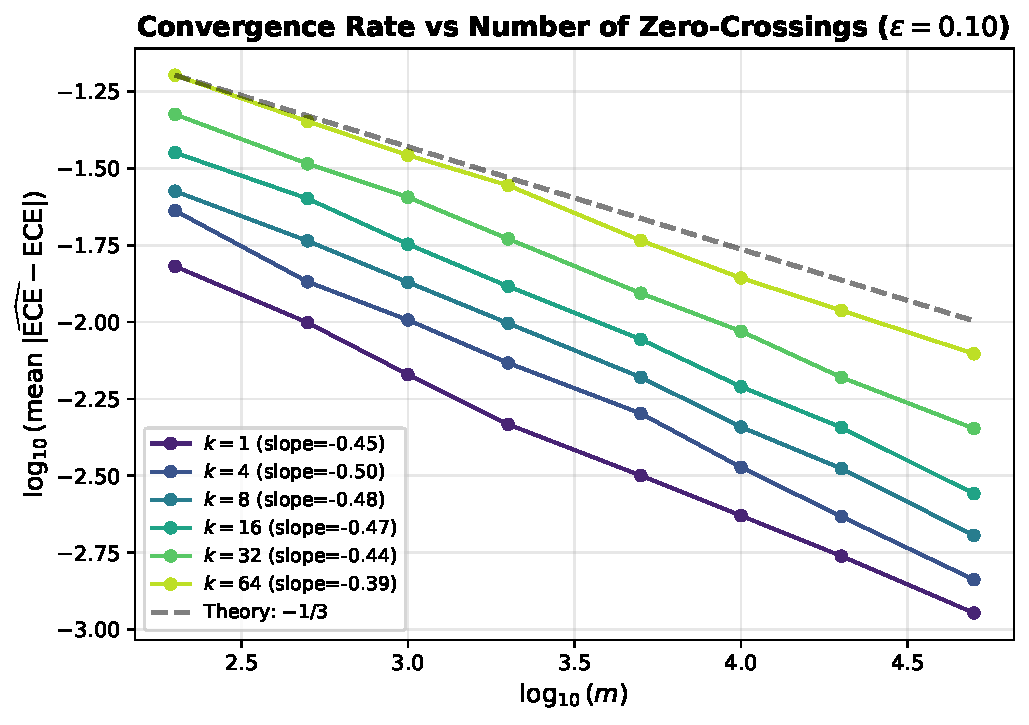
\includegraphics[width=\textwidth]{figures/fig5_slope_vs_k.pdf}
\caption{Synthetic slope study: estimation error versus sample size for increasing numbers of zero-crossings.}
\label{fig:slope-vs-k}
\end{figure}

\begin{figure}[h]
\centering
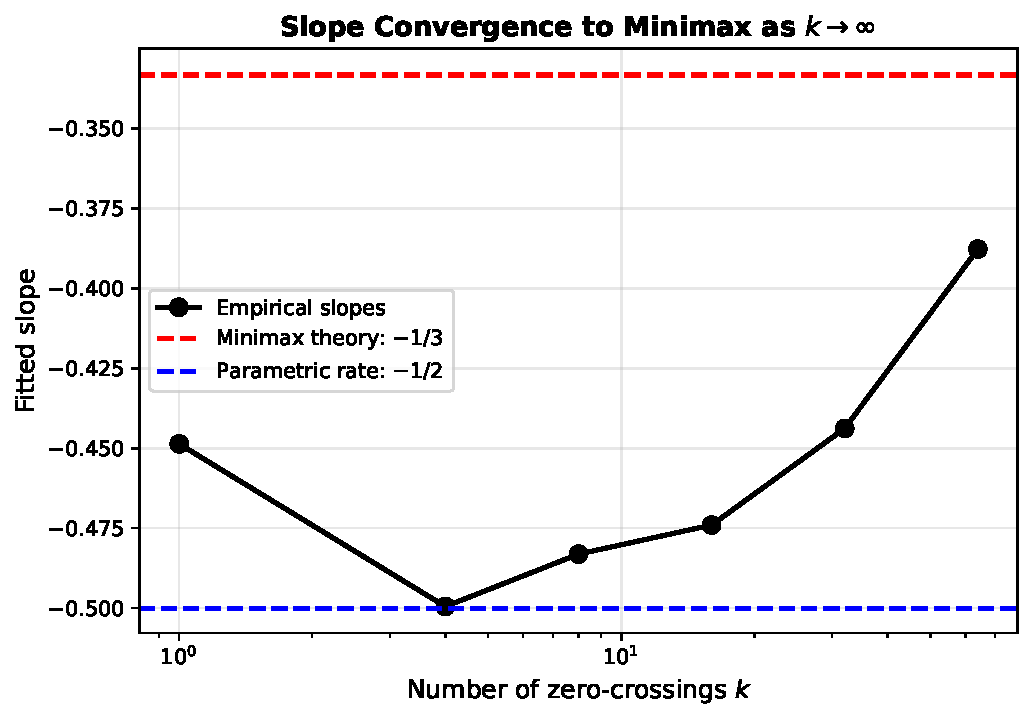
\includegraphics[width=\textwidth]{figures/fig6_slope_convergence.pdf}
\caption{Synthetic slope convergence to the minimax $-1/3$ rate as zero-crossings increase.}
\label{fig:slope-convergence}
\end{figure}

% ============================================================
% SECTION E: Extended Benchmark Analysis + Leaderboard + 5-Benchmark + TruthfulQA + Pipeline (v2)
% ============================================================
\section{Extended Benchmark Analysis}
\label{app:demolition-extended}

\textbf{Leaderboard noise.} Across 57 MMLU subjects, we compute pairwise accuracy gaps between 3 models and compare to per-subject verification floors. Results: 37/57 subjects (65\%) are completely unranked; 56/57 (98\%) have at least one unranked pair; 132/171 pairwise comparisons (77\%) fall below the floor. Mean ranking instability under 80\%-bootstrap: 29.1\%.

\begin{table}[t]
\centering
\caption{Per-subject MMLU rankings for the 20 largest subjects. $\delta_{\mathrm{floor}}$ is the verification floor; gaps below $\delta_{\mathrm{floor}}$ are noise (marked \ding{55}). Instability = fraction of 200 bootstraps where ranking changes.}
\label{tab:leaderboard-noise}
\resizebox{\textwidth}{!}{%
\begin{tabular}{lrccccccc}
\toprule
Subject & $n$ & L405B & L4-Mav & Q3-80B & Max gap & $\delta_{\mathrm{floor}}$ & Verif. & Instab. \\
\midrule
Professional Law & 1534 & 0.72 & 0.68 & 0.68 & 0.040 & 0.175 & \ding{55} & 0.15 \\
Moral Scenarios & 895 & 0.87 & 0.47 & 0.67 & 0.402 & 0.179 & \ding{51} & 0.00 \\
Miscellaneous & 783 & 0.92 & 0.92 & 0.94 & 0.018 & 0.108 & \ding{55} & 0.44 \\
Professional Psychology & 612 & 0.87 & 0.86 & 0.87 & 0.005 & 0.133 & \ding{55} & 0.73 \\
High School Psychology & 545 & 0.93 & 0.92 & 0.96 & 0.037 & 0.104 & \ding{55} & 0.02 \\
High School Macroeconomics & 390 & 0.88 & 0.78 & 0.89 & 0.108 & 0.137 & \ding{55} & 0.27 \\
Elementary Mathematics & 378 & 0.79 & 0.68 & 0.89 & 0.214 & 0.155 & \ding{51} & 0.00 \\
Moral Disputes & 346 & 0.85 & 0.86 & 0.85 & 0.003 & 0.137 & \ding{55} & 0.80 \\
Prehistory & 324 & 0.91 & 0.90 & 0.92 & 0.019 & 0.116 & \ding{55} & 0.46 \\
Philosophy & 311 & 0.86 & 0.85 & 0.85 & 0.016 & 0.136 & \ding{55} & 0.53 \\
High School Biology & 310 & 0.95 & 0.80 & 0.95 & 0.155 & 0.121 & \ding{51} & 0.28 \\
Nutrition & 306 & 0.92 & 0.87 & 0.88 & 0.046 & 0.126 & \ding{55} & 0.43 \\
Professional Accounting & 282 & 0.74 & 0.70 & 0.74 & 0.046 & 0.168 & \ding{55} & 0.48 \\
Professional Medicine & 272 & 0.92 & 0.88 & 0.92 & 0.048 & 0.118 & \ding{55} & 0.47 \\
High School Mathematics & 270 & 0.57 & 0.07 & 0.65 & 0.581 & 0.215 & \ding{51} & 0.00 \\
Clinical Knowledge & 265 & 0.90 & 0.84 & 0.90 & 0.060 & 0.129 & \ding{55} & 0.36 \\
Security Studies & 245 & 0.79 & 0.81 & 0.81 & 0.020 & 0.151 & \ding{55} & 0.55 \\
High School Microeconomics & 238 & 0.95 & 0.89 & 0.95 & 0.063 & 0.107 & \ding{55} & 0.10 \\
High School World History & 237 & 0.92 & 0.93 & 0.93 & 0.008 & 0.108 & \ding{55} & 0.80 \\
Conceptual Physics & 235 & 0.86 & 0.64 & 0.90 & 0.255 & 0.152 & \ding{51} & 0.00 \\
\bottomrule
\end{tabular}}
\end{table}


\section{Extended Empirical Results}
\label{app:extended-empirical}

\textbf{Public-score leaderboard floors.} Table~\ref{tab:leaderboard-floors} summarizes the share of pairwise model comparisons that fall below the accuracy floor across four major public leaderboards plus the technical-report set, computed from public snapshots by \texttt{scripts/exp\_named\_model\_comparison.py}. Full row-level data (model-A, model-B, $n$, $\errrate_A$, $\errrate_B$, gap, floor, verdict per pair) is available in \texttt{results/leaderboard\_floors.csv}.

% Auto-generated by exp_named_model_comparison.py
\begin{table}[t]
\centering
\caption{Share of published pairwise comparisons that fall below the accuracy floor, by leaderboard. Based on snapshot scores; see \texttt{results/leaderboard\_floors.csv} for full data.}
\label{tab:leaderboard-floors}
\small
\begin{tabular}{lrrrr}
\toprule
Leaderboard & Pairs & Unverifiable & Marginal & Verifiable \\
\midrule
AlpacaEval 2.0 (length-controlled) & 6 & 17\% & 17\% & 67\% \\
Chatbot Arena (Arena-Hard-Auto) & 6 & 17\% & 0\% & 83\% \\
HELM (Stanford CRFM) & 10 & 10\% & 10\% & 80\% \\
Open LLM Leaderboard v2 & 10 & 10\% & 10\% & 80\% \\
Tech reports & 13 & 38\% & 15\% & 46\% \\
Tech reports / HELM & 51 & 14\% & 2\% & 84\% \\
\bottomrule
\end{tabular}
\end{table}


\textbf{$\errrate$-dependence comparison against \citet{sun2023recalibration}.} Figure~\ref{fig:sun} reports our passive rate and active rate alongside the $\errrate$-independent upper bound from \citet{sun2023recalibration} at fixed $\nsamples{=}10{,}000$, $\Lip{=}1$. The $2.7\times$ gap at frontier error rates ($\errrate{=}0.05$) and the verification horizon (dashed) illustrate how the $\errrate$-dependence changes the operative regime. The plot is deferred here rather than in the main text because the same comparison is summarized verbally in Section~\ref{sec:empirics}.

\begin{figure}[h]
\centering
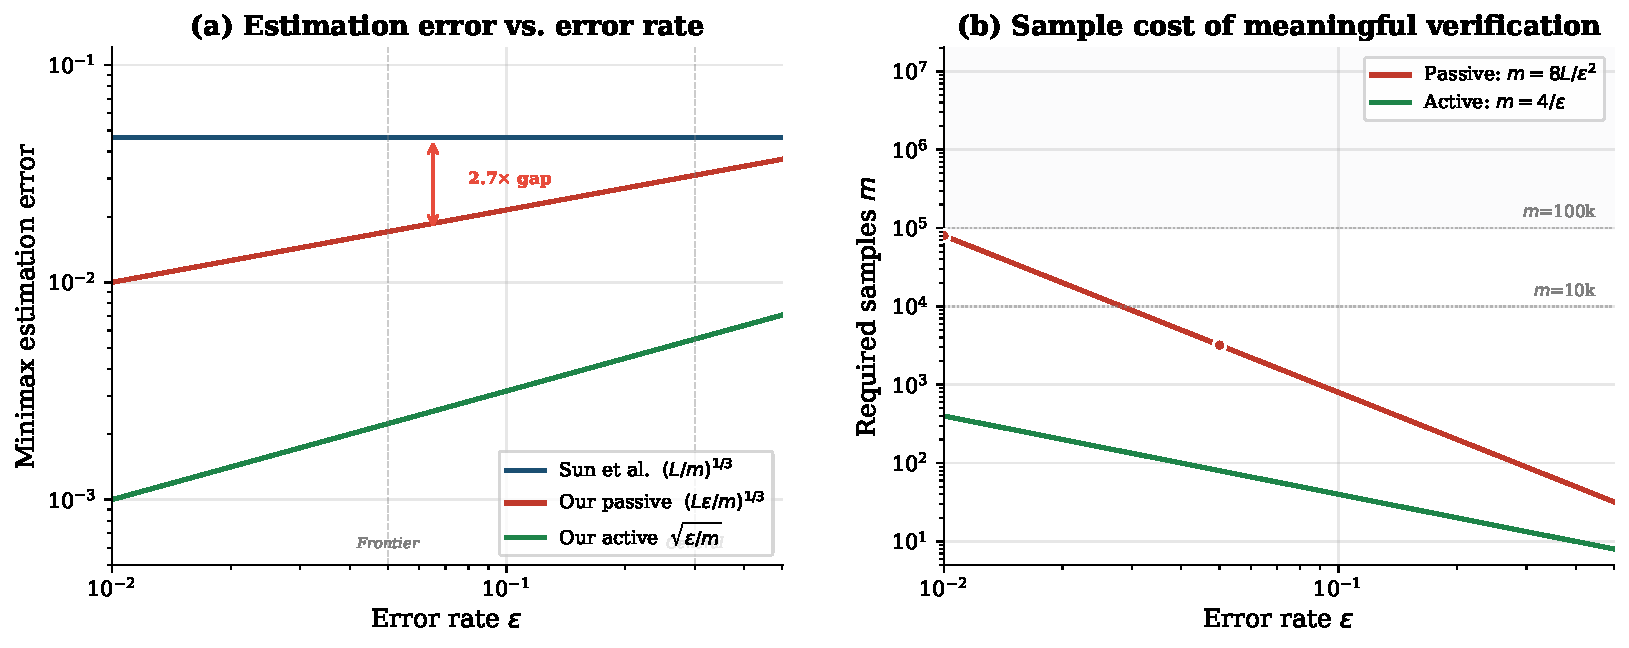
\includegraphics[width=\textwidth]{figures/fig_sun_comparison.pdf}
\caption{\textbf{(a)} Minimax estimation error vs.\ error rate (fixed $\nsamples{=}10{,}000$, $\Lip{=}1$). Sun et al.'s $\errrate$-independent rate is flat; ours decreases with $\errrate$, revealing a $2.7\times$ gap at frontier error rates ($\errrate{=}0.05$). \textbf{(b)} Required samples for meaningful verification ($\targetacc{=}\errrate/2$). Both curves grow as $\errrate \to 0$; the verification horizon (dashed) marks where passive verification exceeds typical benchmark sizes.}
\label{fig:sun}
\end{figure}

\textbf{Screened direct-evidence set.} The saved corpus contains 41 usable benchmark--model runs with at least 100 valid items. Of these, 26 reach at least 70\% benchmark coverage. We then apply the confidence-quality screen described in the main text: minimum confidence standard deviation 0.02, at least 20 unique confidence levels after rounding to 0.001, and no overwhelming fallback mass at 0.25, 0.50, or 1.00. This leaves a 16-pair headline set. The benchmark-by-benchmark breakdown is Table~\ref{tab:screened-roster}.

\begin{table*}[t]
\centering
\caption{Screened headline set for direct item-level calibration claims. Pairs are included only when they have at least 100 valid items, at least 70\% benchmark coverage, and non-degenerate confidence support.}
\label{tab:screened-roster}
\small
\begin{tabular}{llrrcccc}
\toprule
Benchmark & Model & $m$ & Cov. & $\varepsilon$ & ECE & $\hat{L}$ & $\delta_{\mathrm{floor}}$ \\
\midrule
MMLU & Llama 3.1 405B & 14,042 & 100\% & 0.160 & 0.118 & 1.61 & 0.026 \\
MMLU & Llama 4 Maverick & 14,042 & 100\% & 0.273 & 0.262 & 1.00 & 0.027 \\
MMLU & Mistral Small 3.1 & 13,259 & 94\% & 0.223 & 0.157 & 1.26 & 0.028 \\
MMLU & Qwen3 Next 80B & 14,042 & 100\% & 0.165 & 0.143 & 5.00 & 0.039 \\
\midrule
TruthfulQA & Llama 3.1 405B & 817 & 100\% & 0.234 & 0.195 & 2.84 & 0.093 \\
TruthfulQA & Llama 4 Maverick & 817 & 100\% & 0.656 & 0.629 & 3.36 & 0.139 \\
TruthfulQA & Mistral Small 3.1 & 774 & 95\% & 0.229 & 0.166 & 2.69 & 0.093 \\
TruthfulQA & Qwen3 Next 80B & 817 & 100\% & 0.250 & 0.222 & 3.64 & 0.104 \\
\midrule
ARC-Challenge & Llama 3.1 405B & 1,171 & 100\% & 0.053 & 0.045 & 4.18 & 0.057 \\
ARC-Challenge & Llama 4 Maverick & 1,172 & 100\% & 0.047 & 0.044 & 1.00 & 0.034 \\
ARC-Challenge & Mistral Small 3.1 & 1,110 & 95\% & 0.060 & 0.051 & 3.90 & 0.060 \\
ARC-Challenge & Qwen3 Next 80B & 1,172 & 100\% & 0.038 & 0.037 & 1.00 & 0.032 \\
\midrule
HellaSwag & Mistral Small 3.1 & 9,486 & 94\% & 0.069 & 0.047 & 3.06 & 0.028 \\
HellaSwag & Qwen3 Next 80B & 9,447 & 94\% & 0.097 & 0.084 & 5.00 & 0.037 \\
\midrule
WinoGrande & Mistral Small 3.1 & 1,199 & 95\% & 0.220 & 0.180 & 1.68 & 0.068 \\
WinoGrande & Qwen3 Next 80B & 1,198 & 95\% & 0.208 & 0.192 & 5.00 & 0.095 \\
\bottomrule
\end{tabular}
\end{table*}

\textbf{Confidence-quality audit.} High coverage alone is not enough for publication-grade calibration claims. Figure~\ref{fig:confidence-quality} visualizes the problem, and Table~\ref{tab:confidence-quality} lists the excluded high-coverage runs. The excluded runs remain useful for accuracy counting or benchmark-coverage accounting, but their confidence support is too degenerate for statements about calibration shape or self-evaluation.

\begin{figure}[h]
\centering
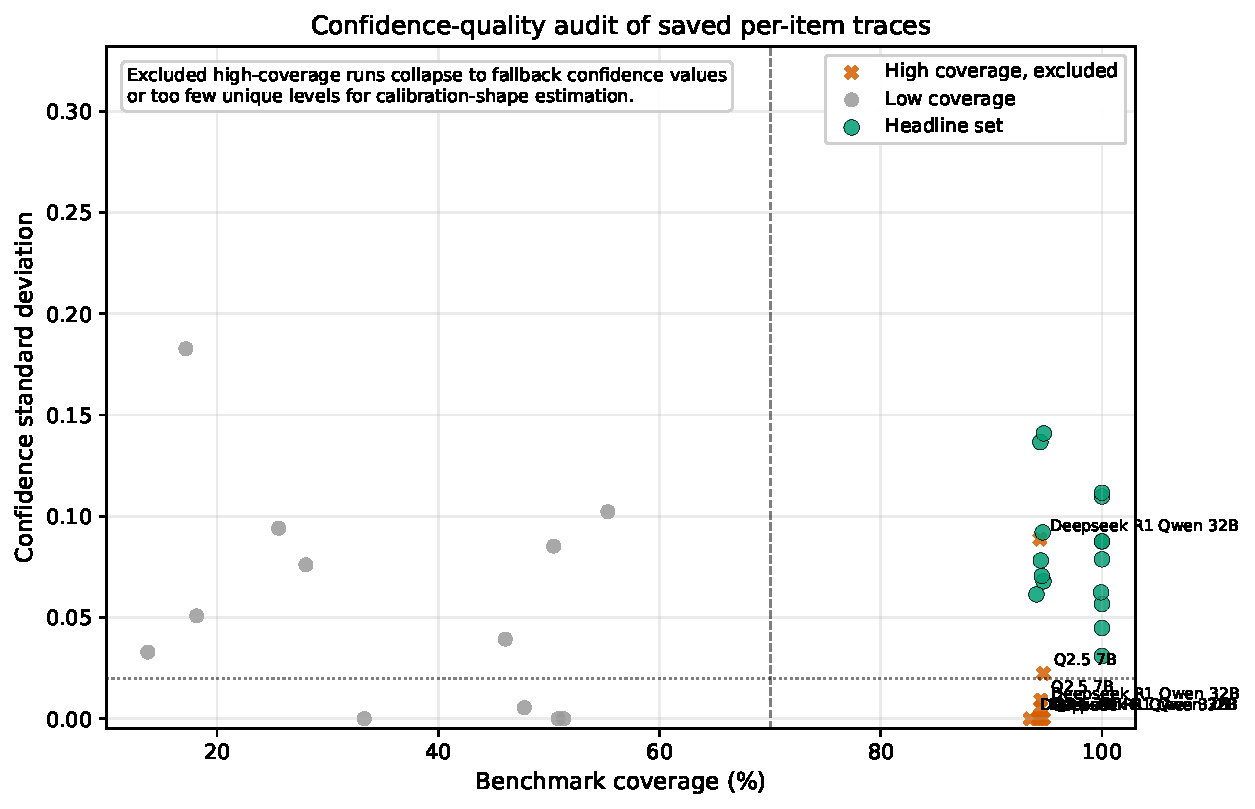
\includegraphics[width=0.82\textwidth]{figures/fig_confidence_quality_audit.pdf}
\caption{Confidence-quality audit for the saved benchmark runs. The headline set requires both high coverage and non-degenerate confidence support. Several high-coverage runs collapse to fallback confidence values and are therefore excluded from direct calibration-shape claims.}
\label{fig:confidence-quality}
\end{figure}

\begin{table*}[t]
\centering
\caption{Confidence-quality audit for high-coverage pairs excluded from the headline set. These runs retain usable accuracy information but their confidence traces are too degenerate for calibration-shape claims.}
\label{tab:confidence-quality}
\footnotesize
\resizebox{\textwidth}{!}{%
\begin{tabular}{p{1.8cm}p{2.6cm}rrp{1.2cm}p{2.0cm}p{4.6cm}}
\toprule
Benchmark & Model & $m$ & Std(conf.) & Unique$_{0.001}$ & Dominant share & Exclusion reason \\
\midrule
MMLU & Deepseek R1 Qwen 32B & 13,128 & 0.000 & 1 & 100\% @ 0.25 & std<0.02; unique<20; dominant>95pct; fallback>95pct \\
MMLU & Qwen2.5 7B & 13,265 & 0.009 & 2 & 100\% @ 1.00 & std<0.02; unique<20; dominant>95pct; fallback>95pct \\
TruthfulQA & Deepseek R1 Qwen 32B & 771 & 0.089 & 12 & 27\% @ 0.25 & unique<20 \\
TruthfulQA & Qwen2.5 7B & 774 & 0.000 & 1 & 100\% @ 1.00 & std<0.02; unique<20; dominant>95pct; fallback>95pct \\
ARC-Challenge & Deepseek R1 Qwen 32B & 1,107 & 0.005 & 3 & 99\% @ 0.25 & std<0.02; unique<20; dominant>95pct; fallback>95pct \\
ARC-Challenge & Qwen2.5 7B & 1,110 & 0.023 & 2 & 100\% @ 1.00 & unique<20; dominant>95pct; fallback>95pct \\
HellaSwag & Deepseek R1 Qwen 32B & 9,467 & 0.000 & 1 & 100\% @ 0.25 & std<0.02; unique<20; dominant>95pct; fallback>95pct \\
HellaSwag & Qwen2.5 7B & 9,487 & 0.000 & 1 & 100\% @ 1.00 & std<0.02; unique<20; dominant>95pct; fallback>95pct \\
WinoGrande & Deepseek R1 Qwen 32B & 1,194 & 0.000 & 1 & 100\% @ 0.50 & std<0.02; unique<20; dominant>95pct; fallback>95pct \\
WinoGrande & Qwen2.5 7B & 1,199 & 0.000 & 1 & 100\% @ 1.00 & std<0.02; unique<20; dominant>95pct; fallback>95pct \\
\bottomrule
\end{tabular}}
\end{table*}

\textbf{Self-evaluation audit.} Among the 13 screened runs with enough occupied bins for the confidence-vs-gap surrogate test, 12 are non-significant. The lone significant case is ARC-Challenge for Llama~3.1~405B, where the benchmark is both small and unusually sharp at the top end. This is why the paper treats the theorem as worst-case and the empirical audit as a screen rather than as a universal monotonicity statement.

\textbf{Real 2-stage pipeline.} Our concrete composition experiment uses Llama~3.1~405B as a screening stage and Qwen3 Next 80B as the second-stage decider on disagreements. The composed system has $\hat\Lip_{\mathrm{sys}} = 3.05$ versus $1.41$ for the single-model baseline and raises the passive floor at $m{=}1000$ by $1.31\times$. Figure~\ref{fig:pipeline-real} shows both the error curves and the system-complexity comparison.

\begin{figure}[h]
\centering
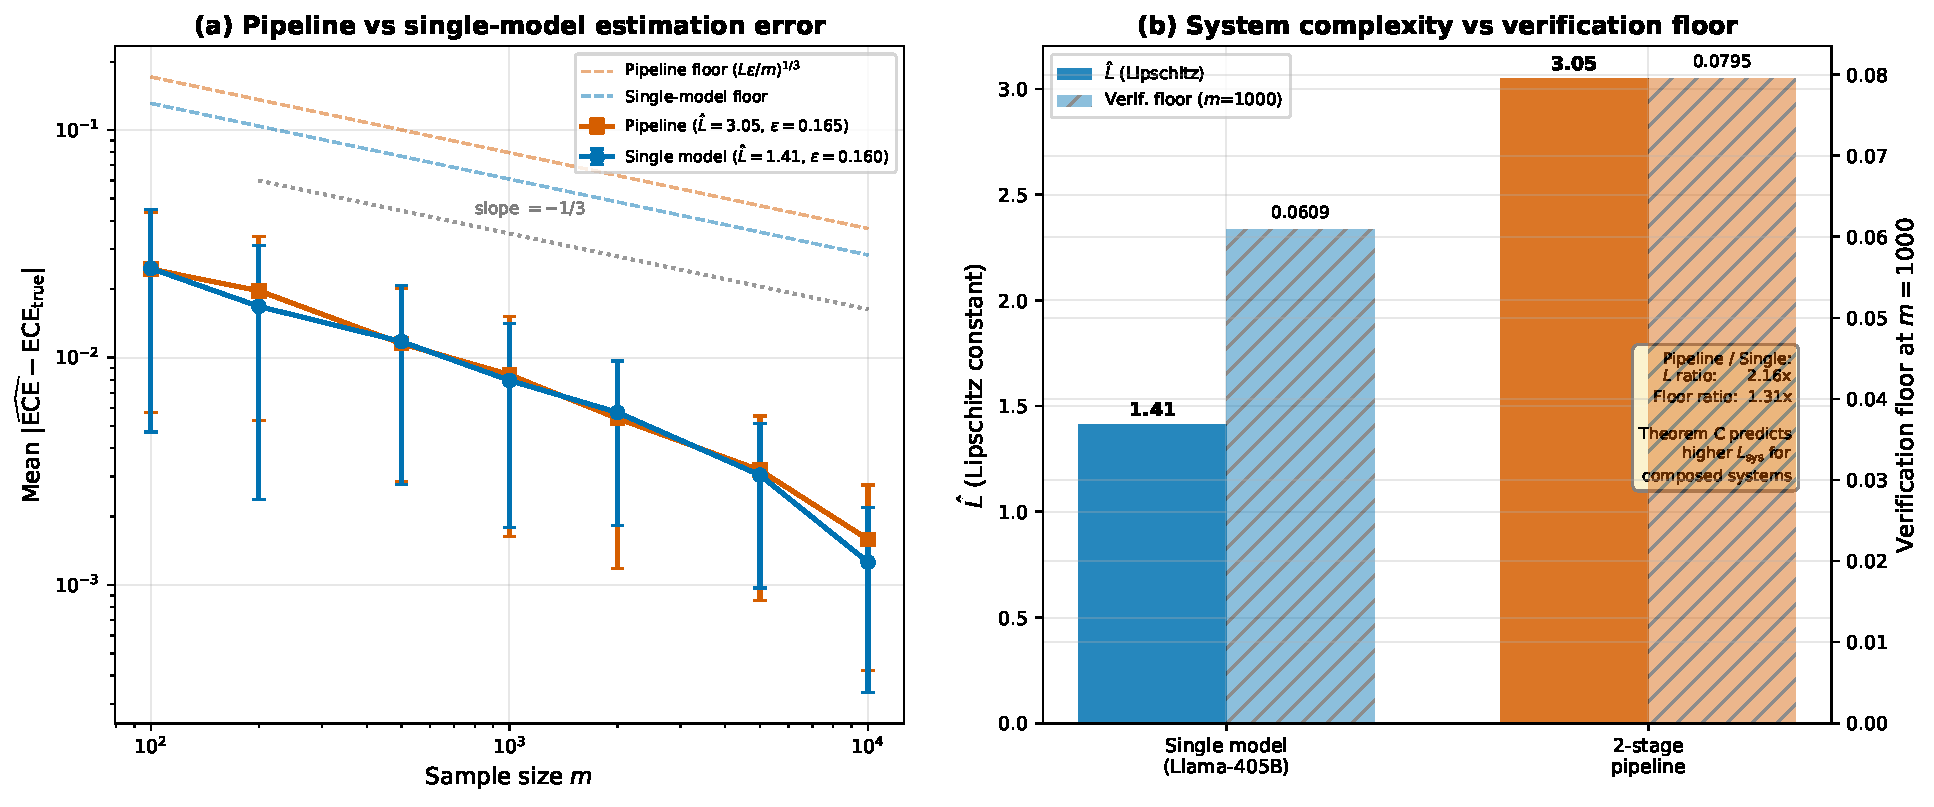
\includegraphics[width=\textwidth]{figures/fig_pipeline_real.pdf}
\caption{Real 2-stage pipeline audit on MMLU. \textbf{Left:} estimation error for the single-model baseline and the composed pipeline. \textbf{Right:} the same experiment viewed through $\hat\Lip$ and the induced passive verification floor.}
\label{fig:pipeline-real}
\end{figure}

\textbf{Measurement and resampling details.} All reported quantities are computed from saved per-item outputs. Coverage is measured against the full benchmark item count. ECE uses the data-dependent optimal bin rule from Theorem~\ref{thm:upper-bound}; $\hat\Lip$ is the 75th percentile of adjacent-bin finite differences, capped at 5. Where bootstrap intervals are shown elsewhere in the appendix, they use 1{,}000 resamples at the item level.

% ============================================================
% SECTION Q: Real-Model Experiment Details (from v1, lines 1126-1149)
% ============================================================
\section{Real-Model Experiment Details}
\label{app:real-model}

\paragraph{MMLU experimental protocol.} We query each NIM-hosted model with the standard 4-way multiple-choice prompt (``Answer the following multiple choice question. Reply with ONLY the letter (A, B, C, or D)''). For each question, we extract the logprobs of the four answer tokens A, B, C, D at the first generated position, apply softmax over those four logits, and take the maximum as the model's confidence. The model's predicted answer is the argmax. Records with API errors (e.g., 403 Forbidden, content-filter rejection) are excluded. Each model run uses a single deterministic temperature-0 generation per question.

\paragraph{Confidence saturation (full data, $N = 14{,}042$ each).} On the complete MMLU set, max-softmax confidence is heavily concentrated near 1: Llama-3.1-405B has mean confidence 0.96 with 77\% of questions saturated ($> 0.99$); Qwen3-Next-80B has mean 0.98 with 86\% saturated; Llama-4-Maverick-17B has mean 0.99 with 92\% saturated. The 405B model has the most spread (lowest saturation rate), as expected for a larger and more capable model. Saturation affects the resolution of high-confidence bins but not the convergence rate, which is governed by the optimal bin count $B^*$.

\paragraph{Lipschitz constant estimation.} For each model, we partition the score range into 20 equal-width bins, compute the empirical accuracy in each bin with at least 30 samples, take the calibration gap $\hat\calmap_b = \mathrm{acc}_b - p_b$ at each bin center, and form the adjacent-bin slope $|\hat\calmap_{b+1} - \hat\calmap_b|/|p_{b+1} - p_b|$. We report the 75th percentile of these slopes, capped at $\hat\Lip = 5$, as a robust estimate. This is sensitive to bin choice and noise; we recommend the audit floor be reported with $\hat\Lip$ from at least two binning resolutions.

\paragraph{Pseudo-classifier control experiment.} As a sanity check before running the real-model experiment, we constructed a 10-class softmax classifier from Gaussian logits with $\errrate \approx 0.10$ ($N = 20{,}000$, full-dataset ECE $\approx 0.31$). Subsampling at $\nsamples \in \{50, \ldots, 10^4\}$ with optimal $B^*$ bins (200 replicates per $\nsamples$) confirms that (i) the verification floor (red dashed in Figure~\ref{fig:pseudo-real-model-error}) tracks the empirical std of estimates across the full range, and (ii) the phase transition near $\nsamples \cdot \errrate \approx 1$ is visible (Figure~\ref{fig:pseudo-real-model-phase}). The pseudo-classifier results match the MMLU real-model findings of Section~\ref{sec:empirics}.

\begin{figure}[h]
\centering
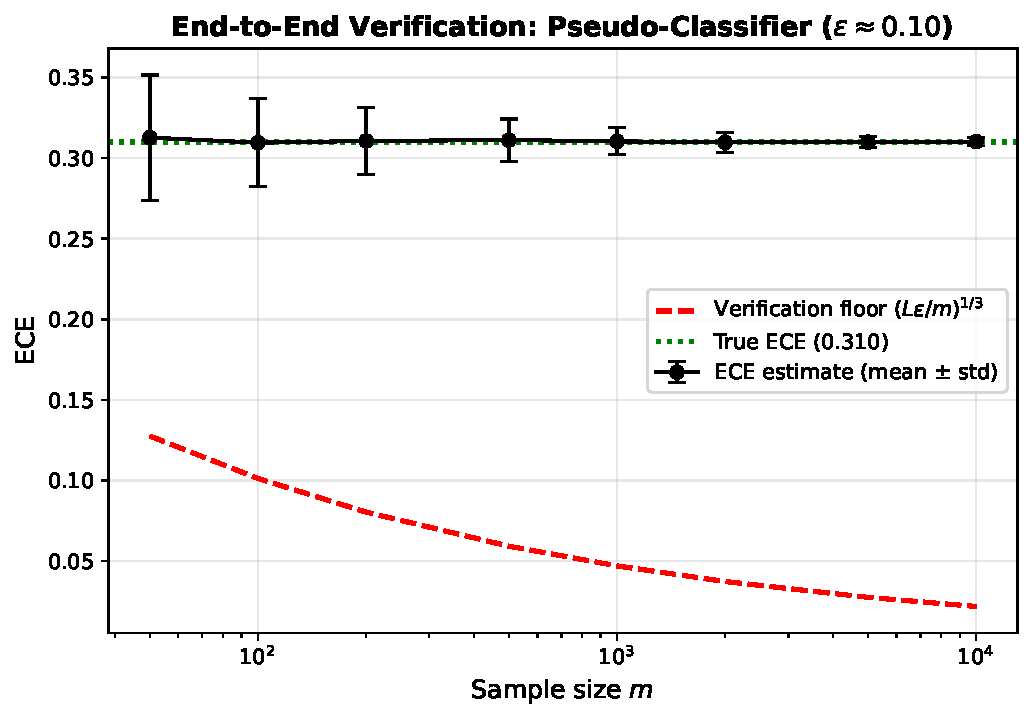
\includegraphics[width=\textwidth]{figures/fig8_real_model.pdf}
\caption{Pseudo-classifier control: ECE estimate $\pm$ std versus $\nsamples$, with the verification floor overlaid.}
\label{fig:pseudo-real-model-error}
\end{figure}

\begin{figure}[h]
\centering
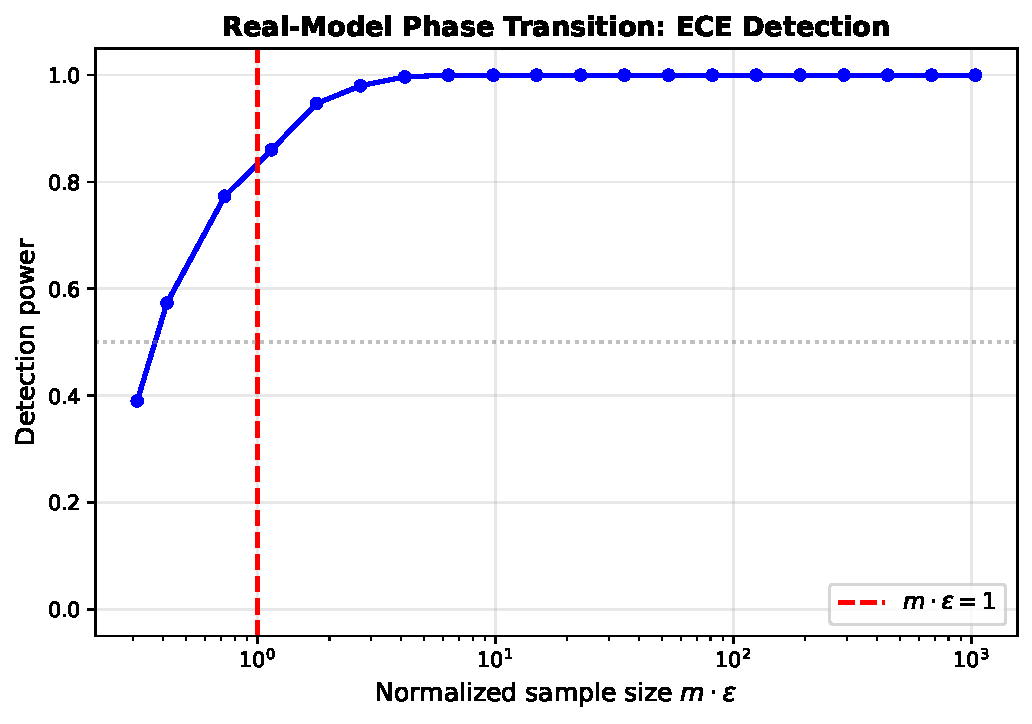
\includegraphics[width=\textwidth]{figures/fig9_real_phase.pdf}
\caption{Pseudo-classifier control: detection power versus $\nsamples \cdot \errrate$, with the predicted phase transition at $\nsamples \cdot \errrate = 1$.}
\label{fig:pseudo-real-model-phase}
\end{figure}

% ============================================================
% SECTION R: Named Model Comparisons (v2 addition)
% ============================================================
\subsection{Named Model Comparisons}
\label{app:named-models}

Full methodology: pairwise accuracy gaps between 10 frontier models on 4 benchmarks using published scores from technical reports and model cards. Verification floor: $\targetacc_{\mathrm{acc}} = 2\sqrt{\errrate(1-\errrate)/n}$. The main-text Table~\ref{tab:named} shows the top comparisons; full data (64 pairs) is in the supplementary materials.

\section{Verification Horizon and Regulatory Tables}
\label{app:horizon-details}

% Auto-generated by exp_verification_horizon.py
\begin{table}[htbp]
\centering
\caption{Verification horizon $N^*$ for frontier models across domains. Gap $= N / N^*$; values $> 1$ indicate the model exceeds the horizon.}
\label{tab:verification_horizon}
\small
\begin{tabular}{llccccc}
\toprule
        Model & Domain & $N$ & $N^*_{\text{pass}}$ & $N^*_{\text{act}}$ & Gap & Exceeds \\
\midrule
        GPT-4                  & General NLP (MMLU-scale)   & $1.80e+12$ & $1.40e+4$ & $1.96e+8$ & 128571428.57 & \cmark \\
        GPT-4                  & Medical imaging            & $1.80e+12$ & $5.00e+5$ & $2.50e+11$ & 3600000.00 & \cmark \\
        GPT-4                  & Legal                      & $1.80e+12$ & $1.00e+4$ & $1.00e+8$ & 180000000.00 & \cmark \\
        GPT-4                  & Financial                  & $1.80e+12$ & $2.00e+4$ & $4.00e+8$ & 90000000.00 & \cmark \\
        GPT-4                  & Code (HumanEval-scale)     & $1.80e+12$ & $5.00e+3$ & $2.50e+7$ & 360000000.00 & \cmark \\
        GPT-4                  & Autonomous driving         & $1.80e+12$ & $1.00e+5$ & $1.00e+10$ & 18000000.00 & \cmark \\
        \addlinespace
        GPT-4o                 & General NLP (MMLU-scale)   & $2.00e+11$ & $1.40e+4$ & $1.96e+8$ & 14285714.29 & \cmark \\
        GPT-4o                 & Medical imaging            & $2.00e+11$ & $5.00e+5$ & $2.50e+11$ & 400000.00 & \cmark \\
        GPT-4o                 & Legal                      & $2.00e+11$ & $1.00e+4$ & $1.00e+8$ & 20000000.00 & \cmark \\
        GPT-4o                 & Financial                  & $2.00e+11$ & $2.00e+4$ & $4.00e+8$ & 10000000.00 & \cmark \\
        GPT-4o                 & Code (HumanEval-scale)     & $2.00e+11$ & $5.00e+3$ & $2.50e+7$ & 40000000.00 & \cmark \\
        GPT-4o                 & Autonomous driving         & $2.00e+11$ & $1.00e+5$ & $1.00e+10$ & 2000000.00 & \cmark \\
        \addlinespace
        Claude 3 Opus          & General NLP (MMLU-scale)   & $1.75e+11$ & $1.40e+4$ & $1.96e+8$ & 12500000.00 & \cmark \\
        Claude 3 Opus          & Medical imaging            & $1.75e+11$ & $5.00e+5$ & $2.50e+11$ & 350000.00 & \cmark \\
        Claude 3 Opus          & Legal                      & $1.75e+11$ & $1.00e+4$ & $1.00e+8$ & 17500000.00 & \cmark \\
        Claude 3 Opus          & Financial                  & $1.75e+11$ & $2.00e+4$ & $4.00e+8$ & 8750000.00 & \cmark \\
        Claude 3 Opus          & Code (HumanEval-scale)     & $1.75e+11$ & $5.00e+3$ & $2.50e+7$ & 35000000.00 & \cmark \\
        Claude 3 Opus          & Autonomous driving         & $1.75e+11$ & $1.00e+5$ & $1.00e+10$ & 1750000.00 & \cmark \\
        \addlinespace
        Claude 3.5 Sonnet      & General NLP (MMLU-scale)   & $7.00e+10$ & $1.40e+4$ & $1.96e+8$ & 5000000.00 & \cmark \\
        Claude 3.5 Sonnet      & Medical imaging            & $7.00e+10$ & $5.00e+5$ & $2.50e+11$ & 140000.00 & \cmark \\
        Claude 3.5 Sonnet      & Legal                      & $7.00e+10$ & $1.00e+4$ & $1.00e+8$ & 7000000.00 & \cmark \\
        Claude 3.5 Sonnet      & Financial                  & $7.00e+10$ & $2.00e+4$ & $4.00e+8$ & 3500000.00 & \cmark \\
        Claude 3.5 Sonnet      & Code (HumanEval-scale)     & $7.00e+10$ & $5.00e+3$ & $2.50e+7$ & 14000000.00 & \cmark \\
        Claude 3.5 Sonnet      & Autonomous driving         & $7.00e+10$ & $1.00e+5$ & $1.00e+10$ & 700000.00 & \cmark \\
        \addlinespace
        Gemini 1.5 Pro         & General NLP (MMLU-scale)   & $5.40e+11$ & $1.40e+4$ & $1.96e+8$ & 38571428.57 & \cmark \\
        Gemini 1.5 Pro         & Medical imaging            & $5.40e+11$ & $5.00e+5$ & $2.50e+11$ & 1080000.00 & \cmark \\
        Gemini 1.5 Pro         & Legal                      & $5.40e+11$ & $1.00e+4$ & $1.00e+8$ & 54000000.00 & \cmark \\
        Gemini 1.5 Pro         & Financial                  & $5.40e+11$ & $2.00e+4$ & $4.00e+8$ & 27000000.00 & \cmark \\
        Gemini 1.5 Pro         & Code (HumanEval-scale)     & $5.40e+11$ & $5.00e+3$ & $2.50e+7$ & 108000000.00 & \cmark \\
        Gemini 1.5 Pro         & Autonomous driving         & $5.40e+11$ & $1.00e+5$ & $1.00e+10$ & 5400000.00 & \cmark \\
        \addlinespace
        Llama-3-405B           & General NLP (MMLU-scale)   & $4.05e+11$ & $1.40e+4$ & $1.96e+8$ & 28928571.43 & \cmark \\
        Llama-3-405B           & Medical imaging            & $4.05e+11$ & $5.00e+5$ & $2.50e+11$ & 810000.00 & \cmark \\
        Llama-3-405B           & Legal                      & $4.05e+11$ & $1.00e+4$ & $1.00e+8$ & 40500000.00 & \cmark \\
        Llama-3-405B           & Financial                  & $4.05e+11$ & $2.00e+4$ & $4.00e+8$ & 20250000.00 & \cmark \\
        Llama-3-405B           & Code (HumanEval-scale)     & $4.05e+11$ & $5.00e+3$ & $2.50e+7$ & 81000000.00 & \cmark \\
        Llama-3-405B           & Autonomous driving         & $4.05e+11$ & $1.00e+5$ & $1.00e+10$ & 4050000.00 & \cmark \\
        \addlinespace
        Llama-4-Maverick       & General NLP (MMLU-scale)   & $1.70e+10$ & $1.40e+4$ & $1.96e+8$ & 1214285.71 & \cmark \\
        Llama-4-Maverick       & Medical imaging            & $1.70e+10$ & $5.00e+5$ & $2.50e+11$ & 34000.00 & \cmark \\
        Llama-4-Maverick       & Legal                      & $1.70e+10$ & $1.00e+4$ & $1.00e+8$ & 1700000.00 & \cmark \\
        Llama-4-Maverick       & Financial                  & $1.70e+10$ & $2.00e+4$ & $4.00e+8$ & 850000.00 & \cmark \\
        Llama-4-Maverick       & Code (HumanEval-scale)     & $1.70e+10$ & $5.00e+3$ & $2.50e+7$ & 3400000.00 & \cmark \\
        Llama-4-Maverick       & Autonomous driving         & $1.70e+10$ & $1.00e+5$ & $1.00e+10$ & 170000.00 & \cmark \\
        \addlinespace
        Qwen3-Next-80B         & General NLP (MMLU-scale)   & $8.00e+10$ & $1.40e+4$ & $1.96e+8$ & 5714285.71 & \cmark \\
        Qwen3-Next-80B         & Medical imaging            & $8.00e+10$ & $5.00e+5$ & $2.50e+11$ & 160000.00 & \cmark \\
        Qwen3-Next-80B         & Legal                      & $8.00e+10$ & $1.00e+4$ & $1.00e+8$ & 8000000.00 & \cmark \\
        Qwen3-Next-80B         & Financial                  & $8.00e+10$ & $2.00e+4$ & $4.00e+8$ & 4000000.00 & \cmark \\
        Qwen3-Next-80B         & Code (HumanEval-scale)     & $8.00e+10$ & $5.00e+3$ & $2.50e+7$ & 16000000.00 & \cmark \\
        Qwen3-Next-80B         & Autonomous driving         & $8.00e+10$ & $1.00e+5$ & $1.00e+10$ & 800000.00 & \cmark \\
\bottomrule
\end{tabular}
\end{table}


% Auto-generated by exp_regulatory_impossibility.py
\begin{table}[htbp]
\centering
\caption{Data requirements for regulatory compliance verification. Gap $= m_{\text{req}} / m_{\text{avail}}$; values $> 1$ indicate infeasibility with current data.}
\label{tab:regulatory_impossibility}
\small
\begin{tabular}{lcccccccc}
\toprule
        Framework & $K$ & $\pi_{\min}$ & $\delta$ & $\varepsilon$ & $m_{\text{req}}$ & $m_{\text{active}}$ & $m_{\text{avail}}$ & Gap \\
\midrule
        EU AI Act Annex III & 10 & 0.05 & 0.020 & 0.050 & $1.25 \times 10^{6}$ & $2.50 \times 10^{4}$ & $7.07 \times 10^{5}$ & 1.8$\times$ \\
        NIST AI RMF & 5 & 0.10 & 0.010 & 0.030 & $1.50 \times 10^{6}$ & $1.50 \times 10^{4}$ & $5.00 \times 10^{5}$ & 3.0$\times$ \\
        FDA SaMD & 8 & 0.05 & 0.010 & 0.020 & $3.20 \times 10^{6}$ & $3.20 \times 10^{4}$ & $7.07 \times 10^{5}$ & 4.5$\times$ \\
\bottomrule
\end{tabular}
\end{table}


\newpage
\section*{NeurIPS Paper Checklist}

\begin{enumerate}

\item {\bf Claims}
    \item[] Question: Do the main claims made in the abstract and introduction accurately reflect the paper's contributions and scope?
    \item[] Answer: \answerYes{}
    \item[] Justification: The abstract and introduction state the four main claims of the paper, and the body and appendix support them with theorems, proof sketches, full proofs, and empirical validation. Scope limits are also stated through the discussion of assumptions and the limitations paragraph near the end of the paper.

\item {\bf Limitations}
    \item[] Question: Does the paper discuss the limitations of the work performed by the authors?
    \item[] Answer: \answerYes{}
    \item[] Justification: The paper includes an explicit ``Limitations and open problems'' paragraph in the conclusion and also notes assumptions and caveats throughout the theory and empirical sections, including Lipschitz assumptions, composition caveats, benchmark-size constraints, and the limitations of provider-managed inference access.

\item {\bf Theory assumptions and proofs}
    \item[] Question: For each theoretical result, does the paper provide the full set of assumptions and a complete (and correct) proof?
    \item[] Answer: \answerYes{}
    \item[] Justification: Theorems in the main text state their assumptions, the main paper provides proof sketches for intuition, and the appendix contains full proofs for the theoretical claims, including the lower bounds, upper bounds, active-verification result, and compositional-verification result.

\item {\bf Experimental result reproducibility}
    \item[] Question: Does the paper fully disclose all the information needed to reproduce the main experimental results of the paper to the extent that it affects the main claims and/or conclusions of the paper (regardless of whether the code and data are provided or not)?
    \item[] Answer: \answerYes{}
    \item[] Justification: The paper specifies the benchmark suite, model roster, prompt and confidence-extraction procedure, finite-difference Lipschitz estimation, bootstrap protocol, permutation tests, and synthetic-experiment setup. The supplementary artifact provides anonymized analysis scripts, derived per-item outputs, saved analysis JSONs, and exact commands for regenerating the main tables and figures from saved outputs.

\item {\bf Open access to data and code}
    \item[] Question: Does the paper provide open access to the data and code, with sufficient instructions to faithfully reproduce the main experimental results, as described in supplemental material?
    \item[] Answer: \answerYes{}
    \item[] Justification: The submission includes an anonymized supplementary artifact with analysis scripts, derived raw result files, saved summaries, and a README containing environment setup and exact reproduction commands. The paper also states explicitly what is included in that anonymous supplementary artifact and what is intentionally excluded.

\item {\bf Experimental setting/details}
    \item[] Question: Does the paper specify all the training and test details (e.g., data splits, hyperparameters, how they were chosen, type of optimizer) necessary to understand the results?
    \item[] Answer: \answerYes{}
    \item[] Justification: The paper documents the benchmark sizes, model families, prompt protocol, score extraction, filtering of API failures, binning procedure for $\hat{\Lip}$, bootstrap setup, permutation testing, and synthetic-data construction. Because the paper studies evaluation rather than training a new model, there are no optimizer or training-hyperparameter choices for a newly trained system to report.

\item {\bf Experiment statistical significance}
    \item[] Question: Does the paper report error bars suitably and correctly defined or other appropriate information about the statistical significance of the experiments?
    \item[] Answer: \answerYes{}
    \item[] Justification: The empirical sections report 95\% bootstrap confidence intervals and permutation tests, and the appendix explains the bootstrap and testing procedures used for the core validation claims.

\item {\bf Experiments compute resources}
    \item[] Question: For each experiment, does the paper provide sufficient information on the computer resources (type of compute workers, memory, time of execution) needed to reproduce the experiments?
    \item[] Answer: \answerNo{}
    \item[] Justification: The paper now discloses that hosted-model inference was run through a provider-managed NIM API and that exact server-side GPU type, memory, and total runtime are not observable through that interface. Because those hardware details are not available for every run, we answer conservatively rather than overstating compute reproducibility.

\item {\bf Code of ethics}
    \item[] Question: Does the research conducted in the paper conform, in every respect, with the NeurIPS Code of Ethics \url{https://neurips.cc/public/EthicsGuidelines}?
    \item[] Answer: \answerYes{}
    \item[] Justification: The work is theoretical and evaluative in nature, focuses on auditing limitations in model verification, and does not introduce a new deployed model or unsafe data-collection procedure. We are not aware of any aspect of the work that conflicts with the NeurIPS Code of Ethics.

\item {\bf Broader impacts}
    \item[] Question: Does the paper discuss both potential positive societal impacts and negative societal impacts of the work performed?
    \item[] Answer: \answerYes{}
    \item[] Justification: The conclusion now includes a dedicated broader-impacts paragraph covering both positive impacts (more honest benchmarking and safer auditing practice) and negative or misuse pathways (using the theory to rationalize weak evaluation or deployment decisions), along with the intended mitigation message.

\item {\bf Safeguards}
    \item[] Question: Does the paper describe safeguards that have been put in place for responsible release of data or models that have a high risk for misuse (e.g., pre-trained language models, image generators, or scraped datasets)?
    \item[] Answer: \answerNA{}
    \item[] Justification: The submission presents theory, evaluation methodology, and lightweight verification utilities; it does not release a new generative model or a high-risk scraped dataset.

\item {\bf Licenses for existing assets}
    \item[] Question: Are the creators or original owners of assets (e.g., code, data, models), used in the paper, properly credited and are the license and terms of use explicitly mentioned and properly respected?
    \item[] Answer: \answerYes{}
    \item[] Justification: The paper cites the benchmark and model sources used in the empirical study, and the manuscript now states that the supplementary artifact redistributes only our code and derived evaluation outputs, not benchmark question text or model weights. This is the main license-sensitive design choice in the submission.

\item {\bf New assets}
    \item[] Question: Are new assets introduced in the paper well documented and is the documentation provided alongside the assets?
    \item[] Answer: \answerYes{}
    \item[] Justification: The supplementary artifact includes a README with environment setup, exact reproduction commands, artifact contents, and limitations, together with the anonymized scripts and derived outputs needed to verify the paper's main empirical claims.

\item {\bf Crowdsourcing and research with human subjects}
    \item[] Question: For crowdsourcing experiments and research with human subjects, does the paper include the full text of instructions given to participants and screenshots, if applicable, as well as details about compensation (if any)?
    \item[] Answer: \answerNA{}
    \item[] Justification: The paper does not report crowdsourcing experiments or research with human subjects.

\item {\bf Institutional review board (IRB) approvals or equivalent for research with human subjects}
    \item[] Question: Does the paper describe potential risks incurred by study participants, whether such risks were disclosed to the subjects, and whether Institutional Review Board (IRB) approvals (or an equivalent approval/review based on the requirements of your country or institution) were obtained?
    \item[] Answer: \answerNA{}
    \item[] Justification: The paper does not involve human-subject research.

\item {\bf Declaration of LLM usage}
    \item[] Question: Does the paper describe the usage of LLMs if it is an important, original, or non-standard component of the core methods in this research? Note that if the LLM is used only for writing, editing, or formatting purposes and does \emph{not} impact the core methodology, scientific rigor, or originality of the research, declaration is not required.
    \item[] Answer: \answerYes{}
    \item[] Justification: The empirical portion of the paper evaluates multiple LLMs directly and describes the hosted-model protocol, prompt format, confidence extraction from logprobs, and benchmark coverage. These details appear in the main empirical sections and the appendix's real-model protocol.

\end{enumerate}


\end{document}
